\chapter{The Riemann Zeta Function}\label{ch:zeta}

\begin{chapterintro}
In Chapter~\ref{ch:intro} we met a list of numbers,
\[
t_1 = 14.134725,\quad t_2 = 21.022040,\quad t_3 = 25.010858,\quad \dots,
\]
and were told that they are the ``heights'' of the zeros of a function built from the primes. This chapter builds that function. It is the Riemann zeta function $\zeta(s)$, defined by a sum over all positive integers,
\[
\zeta(s) = 1 + \frac{1}{2^s} + \frac{1}{3^s} + \frac{1}{4^s} + \cdots .
\]
Euler discovered that this sum over \emph{integers} equals a product over \emph{primes}. That single identity is the bridge between the primes of Chapter~\ref{ch:primes} and everything else in this book, including the prime ``frequencies'' $\log p$ that the paper's arithmetic oracle uses.

There is a twist. The zeros we care about sit at points $s=\tfrac12+it$ where the defining sum does \emph{not} converge. To give a meaning to the statement ``$\zeta(\tfrac12+14.134725\,i)=0$'' we need \emph{analytic continuation}: a way of extending a function beyond the region where its first formula works. We will carry this out completely for $\Re s>0$, using an alternating version of the series, and then take Riemann's functional equation on trust to reach the rest of the complex plane. With the function in hand we will find where its zeros can and cannot lie, state the Riemann hypothesis precisely (it is an open problem), and compute the zeros on a computer.

Where this shows up in the paper: the first sentence of Sec.~I of the paper \cite{soniR1} refers to ``the nontrivial zeros $\rho_n=\tfrac12+it_n$ of the Riemann zeta function''; Sec.~II~A and Appendix~A step~(1) describe computing $t_1,\dots,t_{10^4}$ with \texttt{mpmath}. Every table and figure of the paper is built on these numbers.
\end{chapterintro}

\begin{prerequisites}
\item Chapter~\ref{ch:complex}: complex numbers $s=\sigma+it$, modulus, conjugate, Euler's formula $e^{i\theta}=\cos\theta+i\sin\theta$, the definition $a^s=e^{s\log a}$ for real $a>0$, and $|p^{-s}|=p^{-\sigma}$.
\item Chapter~\ref{ch:series}: convergence of sequences and series, the geometric series (real and complex), divergence of the harmonic series, the integral test and the fact that $\sum k^{-s}$ converges exactly when $s>1$, absolute convergence implies convergence, the alternating series test with its error bound, conditional convergence.
\item Chapter~\ref{ch:asymptotics}: the Gamma function $\Gamma$ as a generalized factorial with $\Gamma(n+1)=n!$; bisection.
\item Chapter~\ref{ch:primes}: primes, Euclid's theorem, the fundamental theorem of arithmetic (every integer $k\ge2$ is a product of primes in exactly one way, up to order).
\item First-year physics and calculus: derivatives, the chain and product rules, improper integrals, small-angle approximations, rotating arrows (phasors).
\end{prerequisites}

%=====================================================================
\section{A sum over all the positive integers}\label{sec:zeta-real}

Imagine a long row of springs, the $k$-th of which contributes an amount $1/k^s$ to some total. If $s$ is large the contributions die off quickly and the total is finite; if $s$ is small they die off so slowly that the total runs away. The zeta function is this total, viewed as a function of the decay exponent $s$.

\paragraph{Definition.} For a real number $s>1$, the \emph{Riemann zeta function} is
\begin{equation}
\zeta(s) \;=\; \sum_{k=1}^{\infty}\frac{1}{k^s}
\;=\; 1+\frac{1}{2^s}+\frac{1}{3^s}+\cdots .
\label{eq:zeta-def}
\end{equation}
Here $k$ runs over the positive integers and $s$ is the variable. Recall from Chapter~\ref{ch:series} (integral test) that this series converges exactly when $s>1$; at $s=1$ it is the harmonic series, which diverges.

\paragraph{How big is $\zeta(s)$?} We can trap $\zeta(s)$ between two simple numbers. Let $f(x)=x^{-s}$ with $s>1$. Its derivative is $f'(x)=-s\,x^{-s-1}<0$, so $f$ is positive and decreasing for $x\ge1$. Take an integer $k\ge2$. For every $x$ in the interval $[k-1,k]$ we have
\[
f(k)\;\le\; f(x)\;\le\; f(k-1)\qquad\text{(because $f$ decreases)} .
\]
Integrate over this interval, which has length 1:
\[
f(k)\;\le\;\int_{k-1}^{k}f(x)\,\dd x\;\le\; f(k-1).
\]
Now add these inequalities for $k=2,3,\dots,K$. The integrals join into one integral from 1 to $K$:
\[
\sum_{k=2}^{K}f(k)\;\le\;\int_{1}^{K}f(x)\,\dd x\;\le\;\sum_{k=1}^{K-1}f(k).
\]
The integral is
\[
\int_1^K x^{-s}\,\dd x=\left[\frac{x^{1-s}}{1-s}\right]_1^K=\frac{K^{1-s}-1}{1-s}=\frac{1-K^{1-s}}{s-1}.
\]
Because $1-s<0$, $K^{1-s}\to0$ as $K\to\infty$, so the integral tends to $1/(s-1)$. Letting $K\to\infty$ in both inequalities (the left sum tends to $\zeta(s)-1$, the right sum to $\zeta(s)$) gives
\[
\zeta(s)-1\;\le\;\frac{1}{s-1}\;\le\;\zeta(s),
\]
which we rearrange as
\begin{equation}
\frac{1}{s-1}\;\le\;\zeta(s)\;\le\;1+\frac{1}{s-1}\qquad (s>1).
\label{eq:zeta-bounds}
\end{equation}
Two consequences are immediate. First, as $s\to1^{+}$, $\zeta(s)$ grows without bound, like $1/(s-1)$. Second, as $s\to\infty$, the upper bound tends to 1 and the lower bound to 0, while every term after the first vanishes; $\zeta(s)\to1$.

The same argument applied to the \emph{tail} $\sum_{k>N}k^{-s}$ (sum the inequalities $\int_k^{k+1}f\le f(k)\le\int_{k-1}^k f$ over $k\ge N+1$) gives
\begin{equation}
\frac{(N+1)^{1-s}}{s-1}\;\le\;\sum_{k=N+1}^{\infty}\frac{1}{k^s}\;\le\;\frac{N^{1-s}}{s-1}.
\label{eq:zeta-tail}
\end{equation}
This tells you how many terms you need for a given accuracy.

\begin{table}[htbp]\centering
\caption{Values of $\zeta(s)$ for real $s$ together with the bounds of \cref{eq:zeta-bounds}. The values for $s=2,4$ are exact formulas (see the box below); all others are computed numerically (CHECKS).}
\label{tab:zeta-values}
\begin{tabular}{cccc}
\toprule
$s$ & lower bound $1/(s-1)$ & $\zeta(s)$ & upper bound $1+1/(s-1)$\\
\midrule
1.5 & 2.000000 & 2.612375 & 3.000000\\
2 & 1.000000 & $\pi^2/6=1.644934$ & 2.000000\\
3 & 0.500000 & 1.202057 & 1.500000\\
4 & 0.333333 & $\pi^4/90=1.082323$ & 1.333333\\
\bottomrule
\end{tabular}
\end{table}

\begin{beyond}
\textbf{Exact values at even integers.} Euler showed in 1735 that $\zeta(2)=\pi^2/6$ (the ``Basel problem''), and more generally that $\zeta(2n)$ is a rational multiple of $\pi^{2n}$, for example $\zeta(4)=\pi^4/90$. We use these values but do not prove them here. If you have read Chapter~\ref{ch:fourier-series}, here is the route for $\zeta(2)$: the function $f(x)=x$ on $(-\pi,\pi)$ has the Fourier series $\sum_{k\ge1}b_k\sin kx$ with $b_k=2(-1)^{k+1}/k$, and Parseval's theorem $\frac1\pi\int_{-\pi}^{\pi}f^2\,\dd x=\sum b_k^2$ reads $\frac{2\pi^2}{3}=\sum_k\frac{4}{k^2}$, which is $\zeta(2)=\pi^2/6$. For odd integers no such formula is known; Ap\'ery proved in 1978 that $\zeta(3)=1.202057\ldots$ is irrational. Proofs are in \cite{apostol} and \cite{edwards}.
\end{beyond}

\begin{sample}{Partial sums of $\zeta(2)$}
Add the first ten terms of $\zeta(2)$, then use \cref{eq:zeta-tail} to trap $\zeta(2)$ in an interval. Is $\pi^2/6$ inside?

\textbf{Step 1:} The partial sum is
\[
S_{10}=1+\tfrac14+\tfrac19+\tfrac1{16}+\tfrac1{25}+\tfrac1{36}+\tfrac1{49}+\tfrac1{64}+\tfrac1{81}+\tfrac1{100}=1.549768 .
\]
\textbf{Step 2:} With $s=2$, $N=10$, \cref{eq:zeta-tail} gives $\frac{1}{11}\le\sum_{k\ge11}k^{-2}\le\frac1{10}$.

\textbf{Step 3:} Adding the tail bounds to $S_{10}$:
\[
1.549768+0.090909\le\zeta(2)\le1.549768+0.1 .
\]
\textbf{Step 4:} So $\boxed{1.640677\le\zeta(2)\le1.649768}$, and $\pi^2/6=1.644934$ lies inside.

Notice how slowly the raw partial sums converge: the tail after $N$ terms is at least $1/(N+1)$, so to get within $10^{-6}$ by brute force you need at least $10^6$ terms. Bounding the tail with an integral is far more efficient than adding more terms.
\end{sample}

\begin{checkpoint}
Without a computer, decide whether $\zeta(1.001)$ is larger or smaller than 1000.
\end{checkpoint}
\checkanswer{Larger (or equal at worst): \cref{eq:zeta-bounds} with $s-1=0.001$ gives $1000\le\zeta(1.001)\le1001$.}

\begin{keyideas}
\item $\zeta(s)=\sum_{k\ge1}k^{-s}$ converges for real $s>1$ and diverges at $s=1$.
\item Comparing the sum with $\int x^{-s}\,\dd x$ traps it: $1/(s-1)\le\zeta(s)\le1+1/(s-1)$.
\item $\zeta(s)\to\infty$ as $s\to1^+$ and $\zeta(s)\to1$ as $s\to\infty$; $\zeta(2)=\pi^2/6$.
\end{keyideas}

%=====================================================================
\section{Complex $s$: a sum of spinning arrows}\label{sec:zeta-complex}

The zeros of the paper live at complex values of $s$, so we must let $s$ be complex. Write
\[
s=\sigma+it,
\]
where $\sigma=\Re s$ (real part) and $t=\Im s$ (imaginary part) are real numbers. Recall from Chapter~\ref{ch:complex} that for a real number $a>0$ we define $a^s=e^{s\log a}$, where $\log$ is the natural logarithm. Apply this to $k^{-s}$:
\begin{align}
k^{-s}&=e^{-s\log k} \notag\\
&=e^{-(\sigma+it)\log k}\notag\\
&=e^{-\sigma\log k}\,e^{-it\log k} &&\text{(since $e^{a+b}=e^ae^b$)}\notag\\
&=k^{-\sigma}\bigl[\cos(t\log k)-i\sin(t\log k)\bigr] &&\text{(Euler's formula)}.
\label{eq:zeta-term}
\end{align}

\paragraph{The picture.} Each term $k^{-s}$ is an arrow in the complex plane of length
\[
|k^{-s}|=k^{-\sigma}
\]
pointing at angle $-t\log k$. Hold $\sigma$ fixed and increase $t$: every arrow rotates clockwise, the $k$-th at angular frequency $\log k$ (radians per unit of $t$). The $k=1$ arrow never moves (since $\log1=0$); the $k=2$ arrow makes one full turn every $2\pi/\log2=9.065$ units of $t$; the $k=3$ arrow every $2\pi/\log3$; and so on. The value $\zeta(s)$ is the tip-to-tail sum of infinitely many shrinking arrows spinning at incommensurate rates. A zero of $\zeta$ is a value of $s$ at which all these arrows add up to exactly nothing. The period $9.065$ will come back: it is the period of the ``prime-2 wave'' (running example RE2) that the paper uses in its continuation probe.

\paragraph{Where the series converges.} The sum of the arrow lengths is
\[
\sum_{k=1}^\infty|k^{-s}|=\sum_{k=1}^{\infty}k^{-\sigma}=\zeta(\sigma),
\]
which is finite exactly when $\sigma>1$. By Chapter~\ref{ch:series}, an absolutely convergent complex series converges. So \cref{eq:zeta-def} defines $\zeta(s)$ for every complex $s$ with $\Re s>1$, a \emph{half-plane}. The triangle inequality, applied to partial sums and then passed to the limit, gives the bound
\begin{equation}
|\zeta(s)|\;\le\;\sum_{k=1}^\infty |k^{-s}|\;=\;\zeta(\sigma)\qquad(\sigma>1).
\label{eq:zeta-modbound}
\end{equation}

\paragraph{Multiplying powers.} For positive integers $k$ and $m$,
\[
(km)^{-s}=e^{-s\log(km)}=e^{-s(\log k+\log m)}=e^{-s\log k}\,e^{-s\log m}=k^{-s}m^{-s}.
\]
We will use this repeatedly.

\begin{pitfall}
The rule $(ab)^s=a^sb^s$ is safe when $a$ and $b$ are \emph{positive real} numbers, because then $\log(ab)=\log a+\log b$ exactly. For complex $a,b$ the logarithm has branches (Chapter~\ref{ch:complex}) and the rule can fail. In this chapter the bases are always positive integers, so we are safe.
\end{pitfall}

\paragraph{Mirror symmetry.} Recall that the conjugate of $e^{x+iy}=e^x(\cos y+i\sin y)$ is $e^x(\cos y-i\sin y)=e^{x-iy}$, that is, $\overline{e^{w}}=e^{\bar w}$. Since $\log k$ is real,
\[
\overline{k^{-s}}=\overline{e^{-s\log k}}=e^{-\bar s\log k}=k^{-\bar s}.
\]
The conjugate of a partial sum is the sum of the conjugates, and conjugation does not change distances ($|\bar a-\bar b|=|a-b|$), so conjugates of convergent sequences converge to the conjugate limit. Therefore
\begin{equation}
\zeta(\bar s)=\overline{\zeta(s)}\qquad(\sigma>1).
\label{eq:zeta-conj}
\end{equation}
Reflecting $s$ in the real axis reflects $\zeta(s)$ in the real axis. In particular $\zeta(s)$ is real when $s$ is real, as it should be.

\paragraph{Analytic functions.} A complex function $f$ is \emph{analytic} on a region (an open, connected set of the complex plane) if at every point $s$ of the region the limit
\[
f'(s)=\lim_{h\to0}\frac{f(s+h)-f(s)}{h}
\]
exists, with the \emph{complex} number $h$ allowed to approach $0$ from any direction. This is a strong demand. For $f(z)=z^2$, $\frac{(z+h)^2-z^2}{h}=2z+h\to2z$, fine. For $f(z)=\bar z$, $\frac{\bar h}{h}$ equals $1$ when $h$ is real and $-1$ when $h$ is imaginary, so no limit exists and $\bar z$ is not analytic, although it is perfectly smooth as a map of the plane.

\begin{beyond}
\textbf{$\zeta$ is analytic for $\Re s>1$.} Each term $k^{-s}=e^{-s\log k}$ is analytic with derivative $-\log k\,k^{-s}$. Because the series converges uniformly on every half-plane $\Re s\ge\sigma_0>1$ (its tail is bounded by the tail of $\zeta(\sigma_0)$, independently of $s$), a theorem of Weierstrass says the sum is analytic and may be differentiated term by term: $\zeta'(s)=-\sum_k \log k\,k^{-s}$. Proof: \cite{titchmarsh}, Chapter~1, or the complex-variable chapters of \cite{rhb}.
\end{beyond}

\begin{sample}{Two arrows at $s=2+3i$}
Find $2^{-s}$ and $3^{-s}$ for $s=2+3i$ in the form $a+ib$, and bound $|\zeta(2+3i)|$ from above.

\textbf{Step 1:} By \cref{eq:zeta-term}, $|2^{-s}|=2^{-2}=0.25$ and $|3^{-s}|=3^{-2}=1/9=0.1111$.

\textbf{Step 2:} The angles are $-3\log2=-2.0794$ rad and $-3\log3=-3.2958$ rad.

\textbf{Step 3:} $2^{-s}=0.25[\cos(2.0794)-i\sin(2.0794)]=0.25[-0.4870-0.8734\,i]$, so $2^{-s}=-0.1217-0.2184\,i$.

\textbf{Step 4:} $3^{-s}=\tfrac19[\cos(3.2958)-i\sin(3.2958)]=\tfrac19[-0.9881+0.1536\,i]$, so $3^{-s}=-0.1098+0.0171\,i$.

\textbf{Step 5:} By \cref{eq:zeta-modbound}, $|\zeta(2+3i)|\le\zeta(2)$:
\[
\boxed{2^{-s}=-0.1217-0.2184\,i,\quad 3^{-s}=-0.1098+0.0171\,i,\quad |\zeta(2+3i)|\le1.644934.}
\]
\end{sample}

\begin{checkpoint}
Does the series \cref{eq:zeta-def} converge at $s=3+100i$? Give an upper bound for $|\zeta(3+100i)|$.
\end{checkpoint}
\checkanswer{Yes, because $\Re s=3>1$ (the size of $t$ is irrelevant). The bound is $|\zeta(3+100i)|\le\zeta(3)=1.202057$. A lower bound follows in \cref{sec:zeta-euler}.}

\begin{keyideas}
\item $k^{-s}=k^{-\sigma}e^{-it\log k}$: an arrow of length $k^{-\sigma}$ rotating at angular frequency $\log k$ in $t$.
\item The series converges absolutely in the half-plane $\Re s>1$, where $|\zeta(s)|\le\zeta(\sigma)$.
\item $\zeta(\bar s)=\overline{\zeta(s)}$; $\zeta$ is analytic for $\Re s>1$.
\end{keyideas}

%=====================================================================
\section{The Euler product: integers from primes}\label{sec:zeta-euler}

Every positive integer is built from primes in exactly one way (Chapter~\ref{ch:primes}). Euler saw in 1737 that this fact can be written as an identity between a sum and a product. Here is the idea with only the primes 2 and 3 and $s=2$:
\[
\Bigl(1+\tfrac1{2^2}+\tfrac1{4^2}+\tfrac1{8^2}+\cdots\Bigr)\Bigl(1+\tfrac1{3^2}+\tfrac1{9^2}+\cdots\Bigr)
=\sum_{a,b\ge0}\frac{1}{(2^a3^b)^2}.
\]
Multiplying out produces exactly one term $1/k^2$ for every integer $k$ of the form $2^a3^b$ (1, 2, 3, 4, 6, 8, 9, 12, \dots), each exactly once because factorizations are unique. Including \emph{all} primes should produce every integer exactly once, that is, $\zeta(2)$.

\paragraph{Statement.} For $\Re s>1$,
\begin{equation}
\zeta(s)=\prod_{p}\frac{1}{1-p^{-s}}\;=\;\lim_{P\to\infty}E_P(s),\qquad
E_P(s)=\prod_{p\le P}\frac{1}{1-p^{-s}},
\label{eq:zeta-euler}
\end{equation}
where the product runs over primes $p$ and $E_P$ is the finite product over primes not exceeding $P$.

\paragraph{Proof.} Fix $s$ with $\sigma=\Re s>1$. We use two sets of integers: $S_P$, the positive integers all of whose prime factors are at most $P$ (this includes $k=1$, which has no prime factors), and $S_{P,J}$, the members of $S_P$ in whose factorization every exponent is at most $J$.

\textbf{(a) Each factor is a geometric series.} Since $|p^{-s}|=p^{-\sigma}\le2^{-\sigma}<\tfrac12<1$, the complex geometric series (Chapter~\ref{ch:series}) gives
\[
\frac{1}{1-p^{-s}}=\sum_{j=0}^{\infty}p^{-js}=\lim_{J\to\infty}\sum_{j=0}^{J}p^{-js}.
\]

\textbf{(b) A finite version of the identity.} Consider the finite product of finite sums
\[
\prod_{p\le P}\ \sum_{j=0}^{J}p^{-js}.
\]
Expanding it (finitely many terms, so ordinary algebra applies) gives one term for each choice of an exponent $j_p\in\{0,\dots,J\}$ for every prime $p\le P$. That term is $\prod_{p\le P}p^{-j_ps}=\bigl(\prod_{p\le P}p^{j_p}\bigr)^{-s}$, using the multiplication rule of \cref{sec:zeta-complex}. The integer $k=\prod p^{j_p}$ belongs to $S_{P,J}$; conversely each $k\in S_{P,J}$ arises from its own factorization, and by uniqueness of factorization from no other choice. Hence
\[
\prod_{p\le P}\ \sum_{j=0}^{J}p^{-js}=\sum_{k\in S_{P,J}}k^{-s}.
\]
For example, with $P=3$, $J=2$:
\[
(1+2^{-s}+4^{-s})(1+3^{-s}+9^{-s})=1+2^{-s}+3^{-s}+4^{-s}+6^{-s}+9^{-s}+12^{-s}+18^{-s}+36^{-s}.
\]

\textbf{(c) Let $J\to\infty$.} On the left, each of the finitely many factors tends to $(1-p^{-s})^{-1}$ by (a), so the left side tends to $E_P(s)$. On the right, the series $\sum_{k\in S_P}k^{-s}$ converges absolutely (its terms are a subset of those of $\zeta$). An element of $S_P$ missing from $S_{P,J}$ has some exponent larger than $J$, hence is at least $2^{J+1}$. So
\[
\Bigl|\sum_{k\in S_P}k^{-s}-\sum_{k\in S_{P,J}}k^{-s}\Bigr|\le\sum_{k\ge 2^{J+1}}k^{-\sigma}\xrightarrow[J\to\infty]{}0,
\]
because this is a tail of the convergent series $\zeta(\sigma)$. Therefore $E_P(s)=\sum_{k\in S_P}k^{-s}$.

\textbf{(d) Let $P\to\infty$.} Every integer $k\le P$ belongs to $S_P$ (its prime factors are at most $k\le P$). So the integers \emph{not} in $S_P$ are all larger than $P$, and
\[
|\zeta(s)-E_P(s)|=\Bigl|\sum_{k\notin S_P}k^{-s}\Bigr|\le\sum_{k>P}k^{-\sigma}\le\frac{P^{1-\sigma}}{\sigma-1},
\]
using \cref{eq:zeta-tail} at the last step (with $N=P$). The right side tends to $0$ as $P\to\infty$, which proves \cref{eq:zeta-euler}. $\blacksquare$

\begin{sample}{Building $\zeta(2)$ prime by prime}
Compute $E_P(2)$ for $P=2,3,5,7,11,13$ and compare the error with the bound of step (d).

\textbf{Step 1:} The factor for prime $p$ at $s=2$ is $1/(1-p^{-2})=p^2/(p^2-1)$: these are $\frac43,\frac98,\frac{25}{24},\frac{49}{48},\frac{121}{120},\frac{169}{168}$.

\textbf{Step 2:} Multiply them in turn (\cref{tab:zeta-euler}).

\textbf{Step 3:} The proof's bound with $\sigma=2$ is $P^{1-2}/(2-1)=1/P$. Every error in the table respects it.

\textbf{Step 4:} With six primes,
\[
\boxed{E_{13}(2)=1.617918,\quad \zeta(2)-E_{13}(2)=0.027016\le\tfrac1{13}=0.076923.}
\]
\end{sample}

\begin{table}[htbp]\centering
\caption{Truncated Euler products at $s=2$, against $\zeta(2)=\pi^2/6=1.644934$.}
\label{tab:zeta-euler}
\begin{tabular}{ccccc}
\toprule
$P$ & factor & $E_P(2)$ & $\zeta(2)-E_P(2)$ & bound $1/P$\\
\midrule
2 & 4/3 & 1.333333 & 0.311601 & 0.500000\\
3 & 9/8 & 1.500000 & 0.144934 & 0.333333\\
5 & 25/24 & 1.562500 & 0.082434 & 0.200000\\
7 & 49/48 & 1.595052 & 0.049882 & 0.142857\\
11 & 121/120 & 1.608344 & 0.036590 & 0.090909\\
13 & 169/168 & 1.617918 & 0.027016 & 0.076923\\
\bottomrule
\end{tabular}
\end{table}

\paragraph{Consequence 1: no zeros in $\Re s>1$.} For each prime, $|1-p^{-s}|\le1+|p^{-s}|=1+p^{-\sigma}$ (triangle inequality). Hence
\[
\frac{1}{|E_P(s)|}=\prod_{p\le P}|1-p^{-s}|\le\prod_{p\le P}(1+p^{-\sigma}).
\]
Expanding the right side as in step (b), with exponents restricted to $0$ or $1$, gives a sum of $k^{-\sigma}$ over some distinct positive integers $k$ (the square-free members of $S_P$), which is at most $\zeta(\sigma)$. So $|E_P(s)|\ge1/\zeta(\sigma)$ for every $P$. Since $E_P(s)\to\zeta(s)$ and the modulus is continuous, $|\zeta(s)|\ge1/\zeta(\sigma)$. Combining with \cref{eq:zeta-modbound}:
\begin{equation}
\frac{1}{\zeta(\sigma)}\;\le\;|\zeta(s)|\;\le\;\zeta(\sigma)\qquad(\sigma=\Re s>1).
\label{eq:zeta-lowerbound}
\end{equation}
\textbf{Theorem (proved): $\zeta(s)\neq0$ whenever $\Re s>1$.} So every zero of $\zeta$, whatever it is, lies in $\Re s\le1$, exactly where our series fails. This is why we will need analytic continuation.

\paragraph{Consequence 2: infinitely many primes.} At $s=1$ the sum diverges; the product must then also run away, and that is impossible with finitely many primes. Here is a version with no limits in $s$. Fix $x\ge2$ and choose an integer $J$ with $2^J\ge x$. Repeating step (b) with real $s=1$,
\[
\prod_{p\le x}\frac{1}{1-1/p}\;\ge\;\prod_{p\le x}\sum_{j=0}^{J}\frac{1}{p^j}=\sum_{k\in S_{x,J}}\frac1k\;\ge\;\sum_{k=1}^{\lfloor x\rfloor}\frac1k.
\]
The first inequality holds because each geometric series of positive terms exceeds its truncation. The last holds because every integer $k\le x$ is in $S_{x,J}$: its primes are at most $x$, and an exponent $j$ satisfies $2^j\le p^j\le k\le x\le2^J$, so $j\le J$. Thus
\begin{equation}
\prod_{p\le x}\Bigl(1-\frac1p\Bigr)^{-1}\;\ge\;\sum_{k\le x}\frac1k .
\label{eq:zeta-primes}
\end{equation}
The right side grows without bound (harmonic series, Chapter~\ref{ch:series}). If there were only finitely many primes, the left side would stop changing once $x$ passed the largest prime, and so would be bounded. Contradiction: there are infinitely many primes. This is a second proof of Euclid's theorem, and the first hint that analytic properties of $\zeta$ encode facts about primes.

\begin{sample}{The product beats the harmonic sum}
Check \cref{eq:zeta-primes} at $x=10$.

\textbf{Step 1:} The primes up to 10 are 2, 3, 5, 7, with factors $\frac{1}{1-1/p}=\frac{p}{p-1}$: $2,\ \frac32,\ \frac54,\ \frac76$.

\textbf{Step 2:} Product: $\frac{2\cdot3\cdot5\cdot7}{1\cdot2\cdot4\cdot6}=\frac{210}{48}=4.375$.

\textbf{Step 3:} Harmonic sum: $1+\frac12+\cdots+\frac1{10}=2.928968$.

\textbf{Step 4:} $\boxed{4.375\ge2.928968}$, as required.
\end{sample}

\begin{figure}[htbp]\centering
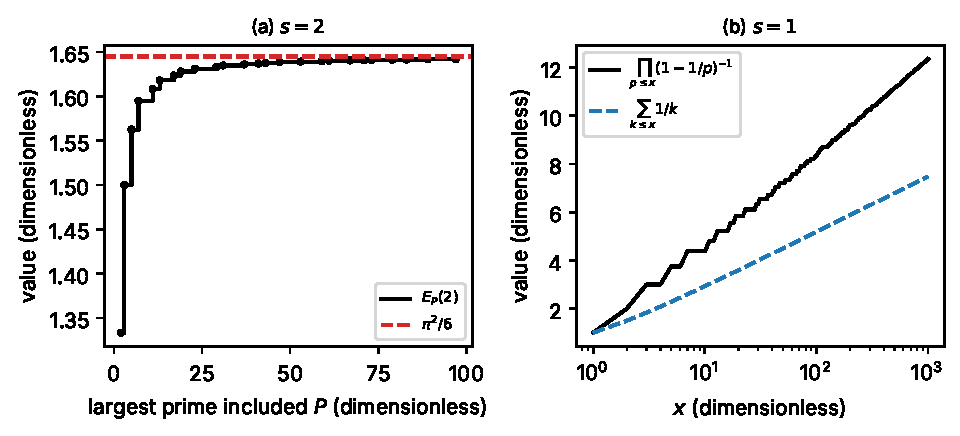
\includegraphics[width=0.85\linewidth]{figs/zeta_euler.pdf}
\caption{The Euler product. (a) Truncated products $E_P(2)$ over primes $p\le P$ approach $\zeta(2)=\pi^2/6$ (dashed) from below as more primes are included. (b) At $s=1$, the product over primes $p\le x$ (solid) stays above the harmonic sum $\sum_{k\le x}1/k$ (dashed), and both grow without bound, so there must be infinitely many primes. All quantities are dimensionless.}
\label{fig:zeta-euler}
\end{figure}

\begin{pitfall}
The Euler product is proved only for $\Re s>1$. On the critical line $\Re s=\tfrac12$, where the zeros live, it does \emph{not} converge, and you cannot locate zeros by asking when a factor vanishes (no factor $(1-p^{-s})^{-1}$ is ever zero). Chapter~\ref{ch:explicit-formula} uses the logarithm of the Euler product \emph{formally} on the critical line to obtain the paper's Eq.~(4); that step is heuristic and is labelled as such there.
\end{pitfall}

\begin{checkpoint}
Using \cref{eq:zeta-lowerbound}, give a lower bound for $|\zeta(3+100i)|$.
\end{checkpoint}
\checkanswer{$|\zeta(3+100i)|\ge1/\zeta(3)=1/1.202057=0.831907$. Together with the earlier checkpoint, $0.831907\le|\zeta(3+100i)|\le1.202057$.}

\begin{keyideas}
\item For $\Re s>1$, $\zeta(s)=\prod_p(1-p^{-s})^{-1}$; the proof is unique factorization plus geometric series.
\item The product shows $\zeta(s)\ne0$ for $\Re s>1$, with $1/\zeta(\sigma)\le|\zeta(s)|\le\zeta(\sigma)$.
\item Divergence at $s=1$ forces infinitely many primes.
\end{keyideas}

%=====================================================================
\section{Analytic continuation}\label{sec:zeta-continuation}

The paper's zeros are at $s=\tfrac12+it_n$. There, $|k^{-s}|=k^{-1/2}$ and $\sum k^{-1/2}$ diverges; our defining series makes no sense. What can ``$\zeta(\tfrac12+14.134725\,i)=0$'' possibly mean? The answer is analytic continuation. We first see it in the simplest possible case.

\subsection{A model: the geometric series}

For complex $z$ with $|z|<1$ the geometric series converges (Chapter~\ref{ch:series}):
\begin{equation}
G(z)=\sum_{k=0}^{\infty}z^k=\frac{1}{1-z}\qquad(|z|<1).
\label{eq:zeta-geom}
\end{equation}
The series defines $G$ only inside the unit disc. The formula $1/(1-z)$, however, makes sense for every $z\ne1$, and it is analytic there: its derivative is $1/(1-z)^2$. Inside the disc the two agree. We say $1/(1-z)$ is the \emph{analytic continuation} of the series to the whole plane minus the point $z=1$. The point $z=1$, where $1/(1-z)$ blows up, is a \emph{pole}.

\begin{figure}[htbp]\centering
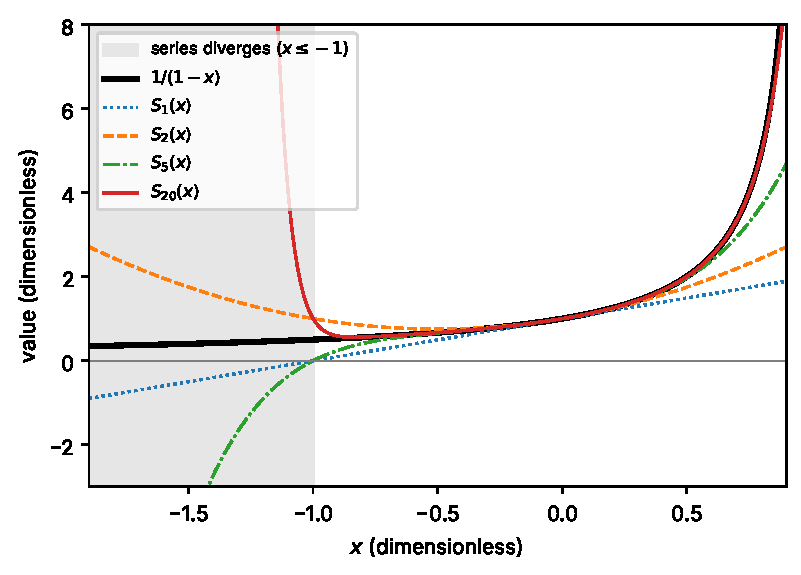
\includegraphics[width=0.85\linewidth]{figs/zeta_geom.pdf}
\caption{Partial sums $S_N(x)=\sum_{k=0}^N x^k$ of the geometric series for real $x$ (thin lines, $N=1,2,5,20$) and the function $1/(1-x)$ (thick). For $-1<x<1$ the partial sums approach $1/(1-x)$; for $x\le-1$ (shaded) they oscillate with growing amplitude and the series diverges, yet $1/(1-x)$ is perfectly finite there. All quantities are dimensionless.}
\label{fig:zeta-geom}
\end{figure}

\begin{sample}{The geometric series at $z=-2$}
Compare the partial sums of $\sum z^k$ at $z=-2$ with $1/(1-z)$.

\textbf{Step 1:} The partial sum of a geometric series is $S_N(z)=\sum_{k=0}^{N}z^k=\frac{1-z^{N+1}}{1-z}$ (Chapter~\ref{ch:series}). At $z=-2$, $S_N(-2)=\frac{1-(-2)^{N+1}}{3}$.

\textbf{Step 2:} The first few are $S_0=1$, $S_1=-1$, $S_2=3$, $S_3=-5$, $S_4=11$: they oscillate with growing size and the series diverges.

\textbf{Step 3:} The continuation is $1/(1-(-2))=1/3$. Note that $S_N=\frac13-\frac{(-2)^{N+1}}{3}$: the continuation is the ``center'' about which the partial sums swing.

\textbf{Step 4:} $\boxed{\text{series diverges; continued value }G(-2)=1/3.}$
\end{sample}

\subsection{Why continuation is unique}

\textbf{Definition.} Let $F$ be analytic on a region $D$. An \emph{analytic continuation} of $F$ to a larger region $D'\supset D$ is a function analytic on $D'$ that equals $F$ on $D$.

You might worry that there are many ways to extend a function, giving many ``values'' at $\tfrac12+14.134725\,i$. For complex-differentiable functions this cannot happen.

\begin{beyond}
\textbf{Identity theorem (uniqueness of analytic continuation).} If two functions are analytic on a connected region and agree on a small disc (or even on a short line segment) inside it, they agree everywhere in the region. Consequently, an analytic continuation, if it exists, is unique: every method of extending $\zeta$ analytically gives the same values. Proof: \cite{titchmarsh}, or the complex-variable chapters of \cite{rhb}. Nothing like this holds for merely smooth real functions: the function equal to $0$ for $x\le0$ and to $e^{-1/x}$ for $x>0$ has derivatives of all orders everywhere, yet agrees with the zero function on $x\le0$ without being zero. Complex differentiability is what rules this out.
\end{beyond}

So the program is: find \emph{some} formula, analytic on a bigger region, that agrees with $\sum k^{-s}$ where the series converges. Uniqueness then makes it \emph{the} zeta function there.

\subsection{The alternating zeta function}

Flip the sign of every second term:
\begin{equation}
\eta(s)=\sum_{k=1}^{\infty}\frac{(-1)^{k+1}}{k^s}=1-\frac1{2^s}+\frac1{3^s}-\frac1{4^s}+\cdots .
\label{eq:zeta-eta}
\end{equation}
This is the \emph{Dirichlet eta function}, or alternating zeta function. Write $S_N(s)=\sum_{k=1}^{N}(-1)^{k+1}k^{-s}$ for its partial sums. The cancellation between neighboring terms makes it converge on a larger region.

\paragraph{Real $s>0$.} The terms $k^{-s}$ are positive, decrease, and tend to $0$. By the alternating series test (Chapter~\ref{ch:series}) the series converges, the partial sums alternate around the limit ($S_2\le S_4\le\cdots\le\eta(s)\le\cdots\le S_3\le S_1$), and
\[
|\eta(s)-S_N(s)|\le(N+1)^{-s}.
\]

\paragraph{Complex $s$ with $\sigma=\Re s>0$.} The alternating series test needs real, decreasing terms, so we need a different argument. We first prove a lemma.

\emph{Lemma.} For real $0<a<b$ and complex $s$,
\begin{equation}
|a^{-s}-b^{-s}|\;\le\;|s|\int_a^b x^{-\sigma-1}\,\dd x .
\label{eq:zeta-etapair}
\end{equation}
\emph{Proof.} Write $x^{-s}=e^{-su}$ with $u=\log x$. The $u$-derivative of $e^{-su}=e^{-\sigma u}[\cos(tu)-i\sin(tu)]$ is, by the product rule,
\[
-\sigma e^{-\sigma u}[\cos tu-i\sin tu]+e^{-\sigma u}[-t\sin tu-it\cos tu]
=-(\sigma+it)\,e^{-\sigma u}[\cos tu-i\sin tu]=-s\,e^{-su},
\]
where in the middle step we used $-t\sin tu-it\cos tu=-it(\cos tu-i\sin tu)$. By the chain rule, $\frac{\dd}{\dd x}x^{-s}=-s\,e^{-su}\cdot\frac1x=-s\,x^{-s-1}$. The fundamental theorem of calculus, applied separately to real and imaginary parts, gives
\[
a^{-s}-b^{-s}=-\int_a^b\frac{\dd}{\dd x}x^{-s}\,\dd x=s\int_a^b x^{-s-1}\,\dd x.
\]
The modulus of an integral of a complex function is at most the integral of its modulus (each Riemann sum obeys the triangle inequality, and the bound survives the limit), and $|x^{-s-1}|=x^{-\sigma-1}$. This gives \cref{eq:zeta-etapair}. $\blacksquare$

\emph{Theorem (proved).} The series \cref{eq:zeta-eta} converges for every complex $s$ with $\Re s>0$.

\emph{Proof.} Group the terms in pairs, $P_j=(2j-1)^{-s}-(2j)^{-s}$ for $j=1,2,\dots$, so that $S_{2J}=\sum_{j=1}^{J}P_j$. By the lemma with $a=2j-1$, $b=2j$,
\[
\sum_{j=1}^{J}|P_j|\le|s|\sum_{j=1}^{J}\int_{2j-1}^{2j}x^{-\sigma-1}\,\dd x\le|s|\int_1^{\infty}x^{-\sigma-1}\,\dd x=\frac{|s|}{\sigma}.
\]
The second inequality holds because the intervals $[2j-1,2j]$ are disjoint pieces of $[1,\infty)$ and the integrand is positive; the integral is $[-x^{-\sigma}/\sigma]_1^\infty=1/\sigma$ since $\sigma>0$. So $\sum_jP_j$ converges absolutely, and $S_{2J}$ tends to a limit, which we call $\eta(s)$. The odd partial sums are $S_{2J+1}=S_{2J}+(2J+1)^{-s}$, and $|(2J+1)^{-s}|=(2J+1)^{-\sigma}\to0$. So $S_N(s)\to\eta(s)$ along all $N$. $\blacksquare$

\begin{pitfall}
For $0<\sigma\le1$ the convergence of $\eta$ is only \emph{conditional}: $\sum|(-1)^{k+1}k^{-s}|=\sum k^{-\sigma}$ diverges. As Chapter~\ref{ch:series} warned, the terms of a conditionally convergent series must be added in their given order; rearranging them can change the sum. Our pairing kept the order, which is why it is legitimate.
\end{pitfall}

\begin{beyond}
\textbf{$\eta$ is analytic on $\Re s>0$.} The pairing argument gives a bound $|s|/\sigma$ that is uniform on any region where $|s|$ is bounded and $\sigma$ is bounded away from $0$; by the same Weierstrass theorem as before, $\eta$ is analytic on the half-plane $\Re s>0$, and in particular continuous there. Proof: \cite{titchmarsh}, Chapter~2.
\end{beyond}

\subsection{From $\eta$ back to $\zeta$}

For $\Re s>1$ both series converge absolutely, and we may subtract them term by term:
\begin{align}
\zeta(s)-\eta(s)&=\sum_{k=1}^\infty\bigl[1-(-1)^{k+1}\bigr]k^{-s}\notag\\
&=\sum_{k\ \mathrm{even}}2\,k^{-s} &&\text{(the bracket is 0 for odd $k$, 2 for even $k$)}\notag\\
&=2\sum_{j=1}^{\infty}(2j)^{-s} &&\text{(write $k=2j$)}\notag\\
&=2\cdot2^{-s}\sum_{j=1}^\infty j^{-s} &&\text{(multiplication rule)}\notag\\
&=2^{1-s}\zeta(s).\notag
\end{align}
Rearranging,
\begin{equation}
\eta(s)=\bigl(1-2^{1-s}\bigr)\,\zeta(s)\qquad(\Re s>1).
\label{eq:zeta-etazeta}
\end{equation}
Now turn this around. The right side of
\begin{equation}
\zeta(s)=\frac{\eta(s)}{1-2^{1-s}}
\label{eq:zeta-cont}
\end{equation}
is defined and analytic for all $\Re s>0$ at which the denominator is not zero, and it agrees with $\sum k^{-s}$ for $\Re s>1$. By uniqueness, \cref{eq:zeta-cont} \emph{is} the zeta function on this larger region. In particular, it is what gives meaning to $\zeta(\tfrac12+14.134725\,i)$.

\paragraph{Where the denominator vanishes.} $1-2^{1-s}=0$ means $e^{(1-s)\log2}=1$. Recall from Chapter~\ref{ch:complex} that $e^{x+iy}=e^x(\cos y+i\sin y)$ equals 1 exactly when $e^x=1$ and $y$ is a multiple of $2\pi$, that is, when $x+iy=2\pi i n$ for an integer $n$. So $(1-s)\log2=2\pi i n$, or
\[
s=1+\frac{2\pi i\,m}{\log 2},\qquad m=0,\pm1,\pm2,\dots
\]
(we renamed $m=-n$). These points lie on the line $\Re s=1$, spaced by $2\pi/\log2=9.0647$ in $t$, the same number as the period of the $2^{-it}$ arrow. At $m=0$ we get $s=1$, discussed next. At $m\ne0$ the formula is $0/0$: $\eta$ also vanishes there (a fact we take on trust here; Problems 25 and 26 give a self-contained proof that $\zeta$ is finite at these points).

\paragraph{The pole at $s=1$.} Near $s=1$ write $u=(s-1)\log2$, a small complex number. Then $2^{1-s}=e^{-u}=1-u+\tfrac{u^2}{2}-\cdots$ (Taylor series of the exponential, Chapter~\ref{ch:complex}), so
\[
1-2^{1-s}=u-\frac{u^2}{2}+\cdots=(s-1)\log2\Bigl[1-\frac{(s-1)\log 2}{2}+\cdots\Bigr].
\]
Meanwhile $\eta$ is continuous at $1$, and $\eta(1)=1-\tfrac12+\tfrac13-\cdots=\log2$. (To see the value: $S_{2n}(1)=\sum_{k=1}^{2n}\frac1k-2\sum_{j=1}^{n}\frac{1}{2j}=\sum_{k=n+1}^{2n}\frac1k$, and comparing with integrals as in \cref{sec:zeta-real}, $\int_{n+1}^{2n+1}\frac{\dd x}{x}\le\sum_{k=n+1}^{2n}\frac1k\le\int_n^{2n}\frac{\dd x}{x}$; both bounds tend to $\log2$.) Hence
\begin{equation}
(s-1)\,\zeta(s)=\frac{(s-1)\,\eta(s)}{1-2^{1-s}}\;\longrightarrow\;\frac{\log 2}{\log2}=1\qquad(s\to1).
\label{eq:zeta-pole}
\end{equation}
So near $s=1$, $\zeta(s)\approx1/(s-1)$. A point $s_0$ where a function behaves like $c/(s-s_0)$ with $c\ne0$ is called a \emph{simple pole} with \emph{residue} $c$. The zeta function has a simple pole at $s=1$ with residue 1, matching the real-variable bounds \cref{eq:zeta-bounds}, which give $1\le(s-1)\zeta(s)\le s$.

\begin{sample}{Close to the pole}
Estimate $\zeta(1.01)$.

\textbf{Step 1:} \cref{eq:zeta-bounds} with $s-1=0.01$: $100\le\zeta(1.01)\le101$.

\textbf{Step 2:} \cref{eq:zeta-pole} predicts $\zeta(1.01)\approx1/0.01=100$, with a correction of order 1 (the bounds say the correction lies between 0 and 1).

\textbf{Step 3:} A computer (\texttt{mpmath.zeta(1.01)}) gives $\zeta(1.01)=100.578$, so $(s-1)\zeta(s)=1.00578$, close to the limit 1.

\textbf{Step 4:} The linearization behind \cref{eq:zeta-pole} can be checked directly: $1-2^{-0.01}=0.0069075$ while $(s-1)\log 2=0.0069315$; they differ by about $0.35\%$, the size of the neglected term $(s-1)\log2/2$.

$\boxed{100\le\zeta(1.01)\le101;\ \zeta(1.01)=100.578.}$
\end{sample}

\begin{sample}{The value $\zeta(\tfrac12)$}
Use \cref{eq:zeta-cont} to find $\zeta(\tfrac12)$, a point where $\sum k^{-s}$ diverges.

\textbf{Step 1:} At $s=\tfrac12$, $2^{1-s}=2^{1/2}=1.414214$, so $1-2^{1-s}=-0.414214$.

\textbf{Step 2:} $\eta(\tfrac12)=1-\frac{1}{\sqrt2}+\frac1{\sqrt3}-\cdots$ converges, slowly: the alternating series bound after $N=1000$ terms is $(1001)^{-1/2}=0.0316$.

\textbf{Step 3:} Because the partial sums alternate around the limit, $\eta$ lies between $S_N$ and $S_{N+1}$, so their average is within half the bound, $0.0158$. In practice the average is far better: averaging $S_{1000}$ and $S_{1001}$ reproduces $\eta(\tfrac12)=0.604899$ to within $10^{-5}$ (\cref{lst:zeta-eta}).

\textbf{Step 4:} $\zeta(\tfrac12)=\eta(\tfrac12)/(1-\sqrt2)=0.604899/(-0.414214)$:
\[
\boxed{\zeta(\tfrac12)=-1.460355.}
\]
The value is \emph{negative}, although every term of $\sum k^{-1/2}$ is positive. There is no contradiction: that series diverges, and $-1.460355$ is the value of the continued function, not a sum.
\end{sample}

\begin{pycode}
import numpy as np

def eta_avg(s, N):
    """Average of the partial sums S_N and S_{N+1} of eta(s)."""
    k = np.arange(1, N + 2)                  # k = 1, ..., N+1
    terms = (-1.0)**(k + 1) * np.exp(-s * np.log(k))
    S = np.cumsum(terms)                     # S[j] = S_{j+1}
    return 0.5 * (S[N - 1] + S[N])

s = 0.5
eta = eta_avg(s, 1000)
print(eta)                                   # about 0.604899
print(eta / (1 - 2**(1 - s)))                # zeta(1/2), about -1.460355
\end{pycode}
\label{lst:zeta-eta}

\begin{figure}[htbp]\centering
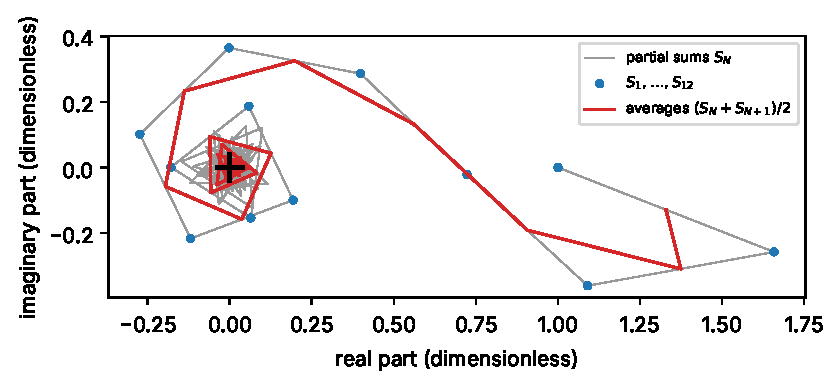
\includegraphics[width=0.85\linewidth]{figs/zeta_eta.pdf}
\caption{Partial sums $S_N$ of the alternating series $\eta(s)$ at $s=\tfrac12+i\,t_1$, $t_1=14.134725$, drawn in the complex plane for $N=1$ to $300$ (gray path; the first twelve partial sums are dots). The averages $(S_N+S_{N+1})/2$ (red) converge much faster. Both head to the origin (cross), because $\eta(\rho_1)=(1-2^{1-\rho_1})\zeta(\rho_1)=0$. Axes are the real and imaginary parts (dimensionless).}
\label{fig:zeta-eta}
\end{figure}

\begin{pitfall}
You may have seen the claim ``$1+2+3+4+\cdots=-\tfrac1{12}$''. The series diverges; it has no sum. What is true is that the analytically continued zeta function satisfies $\zeta(-1)=-\tfrac1{12}$ (we compute it in \cref{sec:zeta-fe}). At $s=-1$ the formula $\sum k^{-s}$ would read $1+2+3+\cdots$, but that formula is not valid there. Never substitute $s$ into $\sum k^{-s}$ unless $\Re s>1$.
\end{pitfall}

\begin{checkpoint}
At $s=1+9.0647\,i$ the denominator $1-2^{1-s}$ in \cref{eq:zeta-cont} is zero. Is $\zeta$ infinite there?
\end{checkpoint}
\checkanswer{No. The numerator $\eta(s)$ also vanishes at these points, and $\zeta$ is finite there; the only pole of $\zeta$ is at $s=1$. Problems 25 and 26 prove this with a second formula whose denominator vanishes at different points.}

\begin{keyideas}
\item Analytic continuation extends a function beyond the domain of its first formula; it is unique (identity theorem).
\item $\eta(s)=\sum(-1)^{k+1}k^{-s}$ converges for $\Re s>0$ and equals $(1-2^{1-s})\zeta(s)$; so $\zeta=\eta/(1-2^{1-s})$ extends $\zeta$ to $\Re s>0$.
\item $\zeta$ has a simple pole at $s=1$ with residue 1: $(s-1)\zeta(s)\to1$.
\item Values like $\zeta(\tfrac12)=-1.460355$ are values of the continuation, not sums of divergent series.
\end{keyideas}

%=====================================================================
\section{The whole plane: the functional equation}\label{sec:zeta-fe}

To reach $\Re s\le0$ we need Riemann's great discovery of 1859 \cite{riemann1859}: a symmetry relating $\zeta(s)$ to $\zeta(1-s)$. It involves the Gamma function. Recall from Chapter~\ref{ch:asymptotics} that $\Gamma$ generalizes the factorial, $\Gamma(n+1)=n!$ for $n=0,1,2,\dots$, and obeys $\Gamma(z+1)=z\,\Gamma(z)$.

\begin{beyond}
\textbf{Facts about $\Gamma$ used here.} The Gamma function extends to all complex $z$ as an analytic function except for simple poles at $z=0,-1,-2,\dots$, and it is never zero. (Proofs in \cite{titchmarsh} and \cite{rhb}.)

\textbf{The functional equation (Riemann, 1859).} The zeta function extends to an analytic function on the whole complex plane except for the simple pole at $s=1$, and for all $s\ne0,1$,
\begin{equation}
\zeta(s)=2^{s}\,\pi^{s-1}\,\sin\!\Bigl(\frac{\pi s}{2}\Bigr)\,\Gamma(1-s)\,\zeta(1-s).
\label{eq:zeta-fe}
\end{equation}
An equivalent, more symmetric form uses $\xi(s)=\tfrac12s(s-1)\pi^{-s/2}\Gamma(s/2)\zeta(s)$, which is analytic everywhere and satisfies
\begin{equation}
\xi(s)=\xi(1-s).
\label{eq:zeta-xi}
\end{equation}
Powers such as $2^s$ and $\pi^{s-1}$ mean $e^{s\log2}$ and $e^{(s-1)\log\pi}$, and $\sin w=(e^{iw}-e^{-iw})/(2i)$ for complex $w$. Proofs: \cite{riemann1859} (original), \cite{edwards} Chapter~1, \cite{titchmarsh} Chapter~2. The CHECKS script verifies \cref{eq:zeta-fe,eq:zeta-xi} numerically at a sample point.
\end{beyond}

\paragraph{How it extends $\zeta$.} If $\Re s<0$, then $\Re(1-s)=1-\Re s>1$, so the right side of \cref{eq:zeta-fe} uses $\zeta(1-s)$ where the original series converges. The equation thus \emph{defines} $\zeta$ on the left half-plane in terms of known values on the right. The strip $0<\Re s<1$ is already covered by \cref{eq:zeta-cont}. The theorem in the box says these pieces join into one analytic function.

\begin{sample}{$\zeta(-1)$ from the functional equation}
Compute $\zeta(-1)$ using \cref{eq:zeta-fe} and $\zeta(2)=\pi^2/6$.

\textbf{Step 1:} Put $s=-1$: $2^{s}=\tfrac12$, $\pi^{s-1}=\pi^{-2}$, $\sin(\pi s/2)=\sin(-\pi/2)=-1$.

\textbf{Step 2:} $\Gamma(1-s)=\Gamma(2)=1!=1$, and $\zeta(1-s)=\zeta(2)=\pi^2/6$.

\textbf{Step 3:} Multiply:
\[
\zeta(-1)=\frac12\cdot\frac1{\pi^2}\cdot(-1)\cdot1\cdot\frac{\pi^2}{6}.
\]
\textbf{Step 4:} The $\pi^2$ cancels: $\boxed{\zeta(-1)=-\tfrac1{12}=-0.083333.}$
\end{sample}

\begin{sample}{$\zeta(0)$ from the pole}
Compute $\zeta(0)$. At $s=0$ the factor $\sin(\pi s/2)$ vanishes while $\zeta(1-s)=\zeta(1)$ is infinite, so we must take a limit.

\textbf{Step 1:} Let $s\to0$. Then $2^s\to1$, $\pi^{s-1}\to1/\pi$, $\Gamma(1-s)\to\Gamma(1)=1$.

\textbf{Step 2:} For small $s$, $\sin(\pi s/2)\approx\pi s/2$ (small-angle approximation; the neglected term is of order $s^3$).

\textbf{Step 3:} Put $u=1-s\to1$. By \cref{eq:zeta-pole}, $(u-1)\zeta(u)\to1$, that is, $(-s)\zeta(1-s)\to1$, so $\zeta(1-s)\approx-1/s$.

\textbf{Step 4:} Multiply: $\zeta(s)\approx\frac1\pi\cdot\frac{\pi s}{2}\cdot1\cdot\Bigl(-\frac1s\Bigr)=-\frac12$. So $\boxed{\zeta(0)=-\tfrac12.}$

By \cref{eq:zeta-etazeta} (which holds wherever both sides are defined, by uniqueness), $\eta(0)=(1-2)\zeta(0)=\tfrac12$: the continued value of $1-1+1-1+\cdots$ is $\tfrac12$, the same as the geometric continuation $1/(1-z)$ at $z=-1$.
\end{sample}

\paragraph{The trivial zeros.} When is $\sin w=0$ for complex $w$? Since $\sin w=(e^{iw}-e^{-iw})/(2i)$, it vanishes exactly when $e^{iw}=e^{-iw}$, that is, $e^{2iw}=1$, that is, $2iw=2\pi i n$, so $w=n\pi$ with $n$ an integer. There are no complex zeros of the sine beyond the familiar real ones. In \cref{eq:zeta-fe}, $\sin(\pi s/2)=0$ exactly when $s$ is an even integer.

Take $s=-2,-4,-6,\dots$, that is $s=-2j$ with $j\ge1$. Then $\sin(-j\pi)=0$, while $2^s\pi^{s-1}$ is finite, $\Gamma(1+2j)=(2j)!$ is finite, and $\zeta(1+2j)$ is a convergent series. Hence
\[
\zeta(-2)=\zeta(-4)=\zeta(-6)=\cdots=0.
\]
These are the \emph{trivial zeros}, ``trivial'' because they come from the sine factor and are completely understood. (At $s=0,2,4,\dots$ the vanishing sine is compensated by a pole: of $\zeta(1-s)$ at $s=0$, as in the sample problem, and of $\Gamma(1-s)$ at $s=2,4,\dots$; so these are not zeros.)

\begin{figure}[htbp]\centering
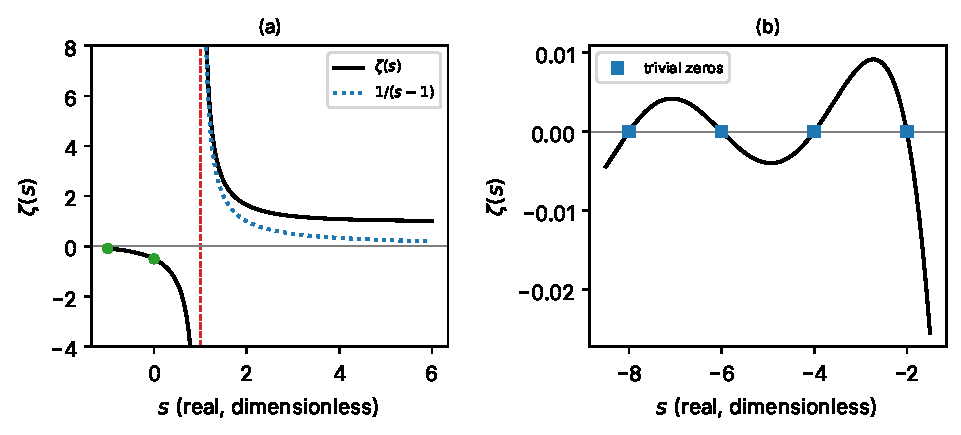
\includegraphics[width=0.85\linewidth]{figs/zeta_real.pdf}
\caption{The continued zeta function on the real axis. (a) $-1\le s\le6$: the simple pole at $s=1$, with $1/(s-1)$ dotted for comparison; $\zeta(0)=-\tfrac12$, $\zeta(-1)=-\tfrac1{12}$, and $\zeta(s)\to1$ for large $s$. (b) Zoom on $-8.5\le s\le-1.5$: the trivial zeros at $s=-2,-4,-6,-8$ (squares). Between them the values are small, for example $\zeta(-3)=1/120$. All quantities are dimensionless.}
\label{fig:zeta-real}
\end{figure}

\begin{checkpoint}
Is $s=-3$ a trivial zero?
\end{checkpoint}
\checkanswer{No. $\sin(-3\pi/2)=+1\ne0$, and the other factors in \cref{eq:zeta-fe} are finite and nonzero, so $\zeta(-3)\ne0$. In fact $\zeta(-3)=\tfrac1{120}$ (Problem 13). Only negative \emph{even} integers are trivial zeros.}

\begin{keyideas}
\item The functional equation $\zeta(s)=2^s\pi^{s-1}\sin(\pi s/2)\Gamma(1-s)\zeta(1-s)$ (taken on trust) extends $\zeta$ to the whole plane, analytic except for the pole at $s=1$.
\item $\zeta(0)=-\tfrac12$, $\zeta(-1)=-\tfrac1{12}$.
\item The trivial zeros are $s=-2,-4,-6,\dots$, from the sine factor.
\end{keyideas}

%=====================================================================
\section{Where the zeros can be}\label{sec:zeta-strip}

We now collect what is known about the location of the zeros of $\zeta$, labelling each statement's status.

\begin{enumerate}
\item \textbf{No zeros in $\Re s>1$.} Theorem, proved in \cref{sec:zeta-euler} from the Euler product.
\item \textbf{In $\Re s<0$ the only zeros are $-2,-4,-6,\dots$.} Theorem, proved here from \cref{eq:zeta-fe} and the $\Gamma$ facts in the box. For $\Re s<0$ each factor on the right of \cref{eq:zeta-fe} is examined: $2^s\pi^{s-1}$ is an exponential, never zero; $\Gamma(1-s)$ is never zero; $\zeta(1-s)\ne0$ by item 1, since $\Re(1-s)>1$; and $\sin(\pi s/2)=0$ only at even integers. So the zeros in $\Re s<0$ are exactly the negative even integers.
\item \textbf{No zeros on the line $\Re s=1$.} Theorem, proved by Hadamard and de la Vall\'ee Poussin in 1896; it is the key step in their proof of the prime number theorem (Chapter~\ref{ch:primes}). The proof is beyond this book; see \cite{davenport} or \cite{titchmarsh}.
\item \textbf{No zeros on the line $\Re s=0$.} Follows from item 3: at $s=it$ with $t\ne0$, \cref{eq:zeta-fe} gives $\zeta(it)$ as a product of nonzero factors, because $\sin(\pi it/2)\ne0$ (the argument $\pi it/2$ is not a real multiple of $\pi$) and $\zeta(1-it)\ne0$ by item 3. At $s=0$, $\zeta(0)=-\tfrac12\ne0$.
\end{enumerate}

Therefore every zero other than the trivial ones lies in the open \textbf{critical strip}
\[
0<\Re s<1 .
\]
These are the \textbf{nontrivial zeros}. The vertical line $\Re s=\tfrac12$ through the middle of the strip is the \textbf{critical line}.

\begin{beyond}
\textbf{There are infinitely many nontrivial zeros; many are on the critical line.} Hardy proved in 1914 that infinitely many zeros lie on the critical line, and Conrey proved in 1989 that more than two fifths of all nontrivial zeros do. Chapter~\ref{ch:counting-zeros} counts the zeros up to height $T$: roughly $\frac{T}{2\pi}\log\frac{T}{2\pi}$ of them. Proofs: \cite{titchmarsh}, Chapters~9--10.
\end{beyond}

\paragraph{Symmetries of the nontrivial zeros.} Two symmetries organize them.

\emph{Mirror (conjugate) symmetry.} For $\Re s>0$, \cref{eq:zeta-cont} gives $\zeta$ as $\eta/(1-2^{1-s})$. Exactly the argument that proved \cref{eq:zeta-conj} shows $\eta(\bar s)=\overline{\eta(s)}$ (term by term, $\overline{k^{-s}}=k^{-\bar s}$), and $\overline{1-2^{1-s}}=1-2^{1-\bar s}$. Dividing, $\zeta(\bar s)=\overline{\zeta(s)}$ throughout $\Re s>0$. So if $\zeta(\rho)=0$ then $\zeta(\bar\rho)=\bar0=0$.

\emph{Reflection symmetry.} For $s$ in the open strip, every factor in \cref{eq:zeta-fe} other than $\zeta(1-s)$ is finite and nonzero: $s$ is not an even integer, so the sine is nonzero; $\Re(1-s)$ lies in $(0,1)$, so $1-s$ is not a pole of $\Gamma$, and $\Gamma$ is never zero; exponentials are never zero. Hence $\zeta(s)=0$ exactly when $\zeta(1-s)=0$.

Combining: if $\rho=\beta+i\gamma$ is a nontrivial zero ($0<\beta<1$), so are
\begin{equation}
\rho=\beta+i\gamma,\qquad \bar\rho=\beta-i\gamma,\qquad 1-\rho=(1-\beta)-i\gamma,\qquad 1-\bar\rho=(1-\beta)+i\gamma .
\label{eq:zeta-quad}
\end{equation}
Off the critical line ($\beta\ne\tfrac12$) these are four distinct points, symmetric about both the real axis and the critical line. On the critical line ($\beta=\tfrac12$) we have $1-\bar\rho=\rho$ and $1-\rho=\bar\rho$, so the four collapse to a conjugate pair $\tfrac12\pm i\gamma$. In particular, a zero on the critical line can move off the line only by splitting into two zeros mirror-symmetric about it.

\begin{figure}[htbp]\centering
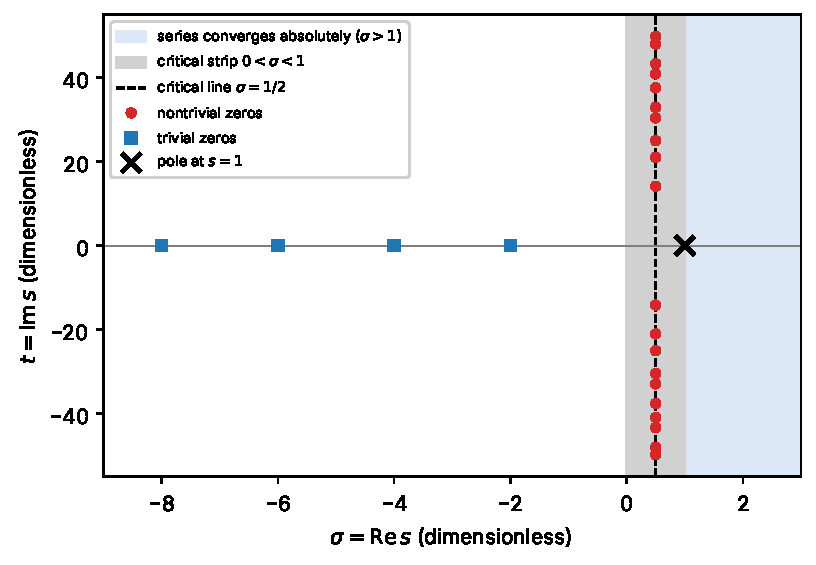
\includegraphics[width=0.85\linewidth]{figs/zeta_strip.pdf}
\caption{Map of the zeta function in the complex $s$ plane, $s=\sigma+it$. The original series converges absolutely for $\sigma>1$ (blue); the critical strip $0<\sigma<1$ (gray) contains all nontrivial zeros; the dashed line is the critical line $\sigma=\tfrac12$. Red dots: the first ten nontrivial zeros $\tfrac12\pm it_n$, $n=1,\dots,10$ (conjugate pairs). Squares: trivial zeros at $-2,-4,-6,-8$. Cross: the pole at $s=1$. Both axes are dimensionless.}
\label{fig:zeta-strip}
\end{figure}

\begin{sample}{Partners of a zero}
(a) List the zeros forced by the first zero $\rho_1=\tfrac12+14.134725\,i$. (b) Suppose, hypothetically, that $\zeta(0.6+20i)=0$. Which other zeros would follow?

\textbf{Step 1:} By \cref{eq:zeta-quad}, (a) gives $\bar\rho_1=\tfrac12-14.134725\,i$, $1-\rho_1=\tfrac12-14.134725\,i$, $1-\bar\rho_1=\tfrac12+14.134725\,i$.

\textbf{Step 2:} Only two of these are distinct: $\tfrac12\pm14.134725\,i$.

\textbf{Step 3:} For (b), $\beta=0.6$, $\gamma=20$: the partners are $0.6-20i$, $0.4-20i$, $0.4+20i$.

\textbf{Step 4:}
\[
\boxed{\text{(a) } \tfrac12\pm14.134725\,i;\qquad\text{(b) } 0.6\pm20i,\ 0.4\pm20i.}
\]
(No zero at $0.6+20i$ exists; the first two zeros above height 20 are at $t=21.022040$ and $25.010858$ on the critical line.)
\end{sample}

\begin{checkpoint}
Why does the paper (and this book) only ever list zeros with $t_n>0$?
\end{checkpoint}
\checkanswer{Because of conjugate symmetry: zeros with negative imaginary part are exactly the mirror images $\bar\rho_n$ of those with positive imaginary part, so they carry no new information. Also there are no zeros on the real segment $0<s<1$ (Problem 22 asks you to explain why).}

\begin{keyideas}
\item Zero-free: $\Re s>1$ (Euler product), $\Re s=1$ and $\Re s=0$ (deep theorem), $\Re s<0$ except $-2,-4,\dots$ (functional equation).
\item Nontrivial zeros lie in the open strip $0<\Re s<1$, in symmetric quadruples $\rho,\bar\rho,1-\rho,1-\bar\rho$, which on the critical line are pairs $\tfrac12\pm i\gamma$.
\end{keyideas}

%=====================================================================
\section{The Riemann hypothesis}\label{sec:zeta-rh}

\paragraph{Statement.} The \textbf{Riemann hypothesis} (RH) is the conjecture:
\begin{center}
\emph{Every nontrivial zero $\rho$ of $\zeta$ has real part exactly $\tfrac12$.}
\end{center}
Equivalently: every zero in the critical strip lies on the critical line.

\paragraph{Status: open.} Riemann wrote in 1859 that it is ``very probable'' that this is so, and that he had put aside the search for a proof \cite{riemann1859,edwards}. It has been neither proved nor disproved since. It is one of the Clay Mathematics Institute's Millennium Prize Problems. Nothing in this book, and nothing in the paper, proves or disproves it.

\paragraph{What is known.}
\begin{itemize}
\item \emph{Proved:} all nontrivial zeros lie in $0<\Re s<1$ (\cref{sec:zeta-strip}); infinitely many lie on the critical line (Hardy, 1914); more than two fifths lie on it (Conrey, 1989).
\item \emph{Reported computational fact:} more than $10^{13}$ zeros, starting from the lowest, have been checked to lie on the critical line and to be simple (large computations were reported by X.~Gourdon in 2004 and by D.~Platt and T.~Trudgian in 2021). This is a finite check, not a proof: it says nothing about zeros higher up.
\item \emph{Numerical observation:} every zero ever computed is simple (not a double zero). That all zeros are simple is a separate open conjecture.
\end{itemize}

\paragraph{Why it matters for primes.} RH is equivalent to the statement that the prime counting function $\pi(x)$ differs from $\mathrm{li}(x)$ (Chapter~\ref{ch:primes}) by at most a constant times $\sqrt{x}\log x$ (a theorem of von Koch, 1901; see \cite{davenport}). The zeros control the fluctuations of the primes, and, as Chapter~\ref{ch:explicit-formula} shows, the primes control the fluctuations of the zeros. This two-way street is the explicit formula behind the paper's oracle.

\paragraph{Notation used from now on.} We list the nontrivial zeros in the upper half-plane by increasing height, $0<t_1<t_2<\cdots$, and write
\[
\rho_n=\tfrac12+i\,t_n .
\]
Writing the real part as $\tfrac12$ is a statement about each \emph{specific} zero we use: each of them has been verified, by the method of \cref{sec:zeta-computing}, to lie on the critical line. It is not an assumption that RH is true in general. The heights $t_n$ are the ``mysterious numbers'' of Chapter~\ref{ch:intro}.

\begin{keyideas}
\item RH: all nontrivial zeros have $\Re\rho=\tfrac12$. It is open.
\item More than $10^{13}$ zeros have been verified on the line (a reported finite computation).
\item We write $\rho_n=\tfrac12+it_n$ with $t_1<t_2<\cdots$ for zeros individually verified on the line.
\end{keyideas}

%=====================================================================
\section{Computing the zeros}\label{sec:zeta-computing}

\subsection{Values and zeros with \texttt{mpmath}}

The Python library \texttt{mpmath} evaluates the continued zeta function at any complex point to any requested precision, using formulas far more efficient than \cref{eq:zeta-cont}. Its function \texttt{mpmath.zetazero(n)} returns the $n$-th zero $\rho_n$ as a complex number.

\begin{pycode}
import mpmath
mpmath.mp.dps = 20                 # work with 20 significant digits

for n in range(1, 11):
    rho = mpmath.zetazero(n)       # complex number 1/2 + i t_n
    print(n, rho.real, mpmath.nstr(rho.imag, 10))

rho1 = mpmath.zetazero(1)
print(abs(mpmath.zeta(rho1)))      # tiny: rho1 really is a zero
\end{pycode}

\begin{table}[htbp]\centering
\caption{The first ten nontrivial zeros (running example RE1) and the gaps between neighbors. Real parts are all $\tfrac12$; the spacings are irregular.}
\label{tab:zeta-zeros}
\begin{tabular}{rcc}
\toprule
$n$ & $t_n$ & $t_{n+1}-t_n$\\
\midrule
1 & 14.134725 & 6.887315\\
2 & 21.022040 & 3.988818\\
3 & 25.010858 & 5.414018\\
4 & 30.424876 & 2.510186\\
5 & 32.935062 & 4.651116\\
6 & 37.586178 & 3.332541\\
7 & 40.918719 & 2.408354\\
8 & 43.327073 & 4.678078\\
9 & 48.005151 & 1.768681\\
10 & 49.773832 & \\
\bottomrule
\end{tabular}
\end{table}

\begin{pitfall}
\texttt{mpmath.zetazero(n)} returns the complex number $\rho_n$, not the height. Use \texttt{.imag} to get $t_n$. Indices start at $n=1$, as in the paper; the book's library \texttt{qmnt.zeros(nmax)} returns the array $t_1,\dots,t_{n_{\max}}$, whose Python index 0 holds $t_1$.
\end{pitfall}

\subsection{The Riemann--Siegel $Z$ function}

How can a computer prove that a zero lies \emph{exactly} on the critical line, when every computed number is rounded? The trick is to find a \emph{real} function whose zeros are the zeros of $\zeta$ on the line. Then the intermediate value theorem does the work: a continuous real function that is negative at one point and positive at another must vanish in between.

Define the Riemann--Siegel theta function and $Z$ function for real $t$:
\begin{align}
\theta(t)&=\Im\log\Gamma\!\Bigl(\frac14+\frac{it}{2}\Bigr)-\frac t2\log\pi, \label{eq:zeta-theta}\\
Z(t)&=e^{i\theta(t)}\,\zeta\!\left(\tfrac12+it\right).\label{eq:zeta-Z}
\end{align}
In \cref{eq:zeta-theta} the imaginary part of $\log\Gamma$ is the phase (argument) of $\Gamma(\tfrac14+\tfrac{it}{2})$, followed continuously from $\theta(0)=0$. Chapter~\ref{ch:counting-zeros} derives from Stirling's formula the approximation $\theta(t)\approx\frac t2\log\frac{t}{2\pi}-\frac t2-\frac\pi8$, which is the origin of the paper's Eq.~(1).

Since $|e^{i\theta}|=1$,
\[
|Z(t)|=|\zeta(\tfrac12+it)|,
\]
so $Z(t)=0$ exactly when $\zeta(\tfrac12+it)=0$. The factor $e^{i\theta(t)}$ rotates $\zeta(\tfrac12+it)$ back onto the real axis.

\begin{beyond}
\textbf{$Z(t)$ is real and continuous for real $t$.} This follows from the functional equation \cref{eq:zeta-xi} together with the mirror symmetry $\zeta(\bar s)=\overline{\zeta(s)}$: on the critical line, $1-s=\bar s$, and the phase of $\zeta(\tfrac12+it)$ is exactly $-\theta(t)$ modulo $\pi$. Proof: \cite{edwards}, Chapter~6; \cite{titchmarsh}, Chapter~4. The CHECKS script confirms numerically that $\Im Z(t)$ vanishes to working precision. In \texttt{mpmath} the functions are \texttt{siegeltheta(t)} and \texttt{siegelz(t)}.
\end{beyond}

At $t=0$, $\theta(0)=0$ and $Z(0)=\zeta(\tfrac12)=-1.460355<0$. Because $Z$ is continuous and has no zeros below $t_1$, it stays negative on $[0,t_1)$; it changes sign at each simple zero.

\begin{figure}[htbp]\centering
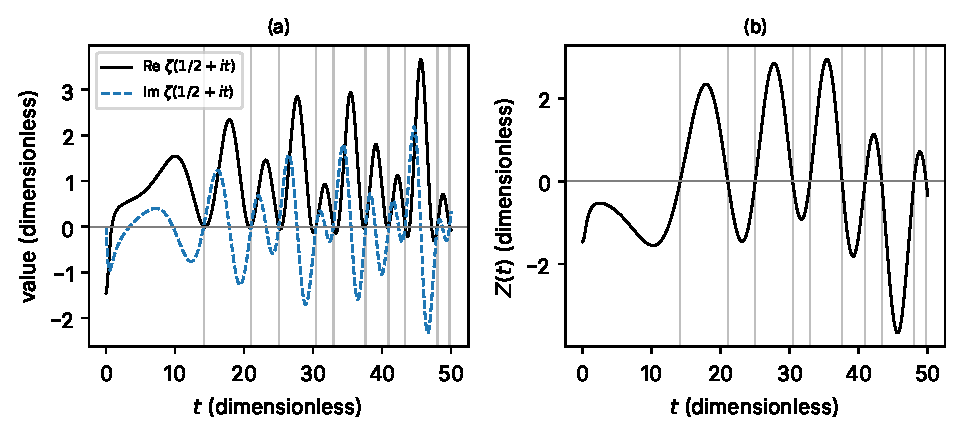
\includegraphics[width=0.85\linewidth]{figs/zeta_Z.pdf}
\caption{The zeta function on the critical line, $0\le t\le50$. (a) Real part (solid) and imaginary part (dashed) of $\zeta(\tfrac12+it)$; at a zero both vanish together (gray lines mark $t_1,\dots,t_{10}$). (b) The Riemann--Siegel function $Z(t)$, a real function with $|Z(t)|=|\zeta(\tfrac12+it)|$, which changes sign at every zero. The variable $t$ and the function values are dimensionless.}
\label{fig:zeta-Z}
\end{figure}

\begin{sample}{Trapping the first zero by bisection}
Given only that $Z(14)<0$ and $Z(15)>0$, locate $t_1$ by eight steps of bisection (Chapter~\ref{ch:asymptotics}), and bound the error.

\textbf{Step 1:} Start with $[a,b]=[14,15]$. At each step evaluate $Z$ at the midpoint $m$ and keep the half on which $Z$ changes sign.

\textbf{Step 2:} The eight steps are listed in \cref{tab:zeta-bisect}. (The signs follow from $t_1=14.134725$: $Z<0$ below it and $Z>0$ above it, up to $t_2=21.02$. The \texttt{mpmath} values agree; see the listing below.)

\textbf{Step 3:} After eight halvings the bracket has width $1/2^8=0.00390625$; its midpoint is $14.134765625$, within half the width, $0.001953$, of the zero.

\textbf{Step 4:}
\[
\boxed{t_1\approx14.134766,\ \text{true error }4.0\times10^{-5}\le0.001953.}
\]
Each step gains one binary digit; about 20 more steps would reach $10^{-6}\times$ the starting width, and since the sign changes of a real function are certain, this \emph{proves} there is a zero exactly on the critical line in the final bracket.
\end{sample}

\begin{table}[htbp]\centering
\caption{Bisection for the first zero on $[14,15]$.}
\label{tab:zeta-bisect}
\begin{tabular}{cccc}
\toprule
step & midpoint $m$ & sign of $Z(m)$ & new bracket\\
\midrule
1 & 14.5 & $+$ & $[14,\ 14.5]$\\
2 & 14.25 & $+$ & $[14,\ 14.25]$\\
3 & 14.125 & $-$ & $[14.125,\ 14.25]$\\
4 & 14.1875 & $+$ & $[14.125,\ 14.1875]$\\
5 & 14.15625 & $+$ & $[14.125,\ 14.15625]$\\
6 & 14.140625 & $+$ & $[14.125,\ 14.140625]$\\
7 & 14.1328125 & $-$ & $[14.1328125,\ 14.140625]$\\
8 & 14.13671875 & $+$ & $[14.1328125,\ 14.13671875]$\\
\bottomrule
\end{tabular}
\end{table}

\begin{pycode}
import mpmath

a, b = 14.0, 15.0
Za = mpmath.siegelz(a)                 # negative
for step in range(1, 9):
    m = 0.5 * (a + b)
    Zm = mpmath.siegelz(m)
    if Zm * Za < 0:                    # sign change in [a, m]
        b = m
    else:                              # sign change in [m, b]
        a, Za = m, Zm
    print(step, m, "+" if Zm > 0 else "-", (a, b))
print("estimate", 0.5 * (a + b))
\end{pycode}

\paragraph{How RH is checked numerically.} Sign changes of $Z$ on $[0,T]$ give a \emph{lower bound} on the number of zeros on the critical line up to height $T$. They can miss zeros only in pairs (two close zeros between sample points) or zeros of even multiplicity. Separately, the argument principle (Chapter~\ref{ch:counting-zeros}) gives the \emph{total} number $N(T)$ of zeros in the whole strip up to height $T$, wherever they are. If the two numbers agree, every zero up to height $T$ is on the critical line and simple. This is the logic of the large verifications (made rigorous with a method due to Turing), and \texttt{mpmath.zetazero} locates zeros with the same ingredients: sign changes of $Z$, organized with the help of the counting function, followed by refinement.

\begin{checkpoint}
Your program finds $Z(30)<0$ and $Z(31)>0$. What can you conclude, and what can you not conclude?
\end{checkpoint}
\checkanswer{You can conclude that there is at least one zero of $\zeta$ exactly on the critical line with $30<t<31$ (here it is $t_4=30.424876$). You cannot conclude that there is only one: an odd number of zeros, counted with multiplicity, lies in the interval. Nor do sign changes say anything about zeros off the line; that needs the count $N(T)$ of Chapter~\ref{ch:counting-zeros}.}

\begin{keyideas}
\item \texttt{mpmath.zeta} evaluates the continued function; \texttt{mpmath.zetazero(n)} returns $\rho_n$.
\item $Z(t)=e^{i\theta(t)}\zeta(\tfrac12+it)$ is real, with $|Z|=|\zeta|$ on the line; its sign changes prove zeros exactly on the critical line.
\item Sign changes plus the zero count $N(T)$ verify RH up to height $T$, a finite check.
\end{keyideas}

%=====================================================================
\section{Paper connection}\label{sec:zeta-paper}

This chapter supplies the objects that the paper \cite{soniR1} takes as its data. Here is where each idea appears.

\paragraph{Sec.~I, first sentence.} ``The Hilbert--P\'olya conjecture proposes that the imaginary parts $t_n$ of the nontrivial zeros $\rho_n=\tfrac12+it_n$ of the Riemann zeta function are the spectrum of a self-adjoint operator.'' You can now read every word. ``Nontrivial'' excludes the zeros $-2,-4,\dots$ of \cref{sec:zeta-fe}; these play no role in the paper. ``$\rho_n=\tfrac12+it_n$'' records that each zero used lies on the critical line, which is verified for every zero in the paper's range (at most $10^4$ zeros, far inside the more than $10^{13}$ checked; \cref{sec:zeta-rh}). The Hilbert--P\'olya idea, developed in Chapter~\ref{ch:hilbert-polya}, is a proposed route to RH: a self-adjoint operator has real eigenvalues (Chapter~\ref{ch:schrodinger}), so if the $t_n$ were its eigenvalues, every $\rho_n$ would have real part exactly $\tfrac12$. RH and Hilbert--P\'olya are both open, and the paper does not claim otherwise; Sec.~VI states that ``Nothing here touches the analytic Hilbert--P\'olya program.''

\paragraph{Sec.~II~A and Appendix~A step (1): the data.} The paper computes ``zeros $t_1,\dots,t_{1000}$ \dots\ with \texttt{mpmath} at 20 significant digits ($t_1=14.134725141734695$, $t_{1000}=1419.42248094599$) and zeros $10^3$--$10^4$ at 15 digits'', via \texttt{mpmath.zetazero(n)} (Appendix~A, step~1). The ``key anchors'' in Appendix~A add $t_{500}=811.1843588465$. These are exactly the computations of \cref{sec:zeta-computing}, and the CHECKS script of this chapter reproduces $t_1$, $t_{500}$ and $t_{1000}$ to the digits printed. A small reading lesson: to 20 digits, $t_1=14.13472514173469379\ldots$; the paper's printed $14.134725141734695$ agrees with it to about $10^{-15}$, the resolution of a double-precision number near 14 (Chapter~\ref{ch:asymptotics}). The paper notes that ``both precisions exceed every use below by many orders'': errors in the paper are quoted in units of the local mean spacing, which near $t_{1000}$ is about 1.159 (Chapter~\ref{ch:counting-zeros}; Problem 21), and the smallest error the paper quotes is an rms below $10^{-4}$ spacings (Sec.~III).

\paragraph{Only positive heights.} By the mirror symmetry of \cref{sec:zeta-strip}, the zeros below the real axis are the conjugates $\bar\rho_n$, so the paper's list $t_1<t_2<\cdots$ of positive heights is the complete information. Every figure of the paper (Fig.~1: fluctuations of zeros 370--460; Fig.~2: spacings of the first $10^4$ zeros) and every table (Tables~I--V, with holdouts up to zero $10^4$ in Table~V) uses this list.

\paragraph{The Euler product behind the oracle.} The paper's arithmetic oracle, Eq.~(4), is a sum of terms $\sin(mt\log p)/(m\,p^{m/2})$ over primes $p$ and powers $m$. You have now seen where $\log p$ and $p^{-1/2}$ come from: by \cref{eq:zeta-term}, the prime factor $p^{-s}$ on the critical line is an arrow of length $p^{-1/2}$ rotating at angular frequency $\log p$ in $t$. Chapter~\ref{ch:explicit-formula} turns the Euler product \cref{eq:zeta-euler} into Eq.~(4) by a formal (heuristic) step; the paper itself says the formula ``has no fitted parameters and no novelty'' (Sec.~II~D). The arrow for $p=2$ turns once every $2\pi/\log 2=9.0647$ in $t$, which is the ``period $2\pi/\log 2\approx 9$ in $t$'' of Sec.~V and the target of the continuation probe in Sec.~III.

\paragraph{Prime-only constructions.} Sec.~I~A(b) and Sec.~II~D cite Connes \cite{connes26}: ``extremizing the truncated Weil quadratic form over primes $p\le13$ yields approximations to the first 50 zeros with accuracies from $10^{-3}$ down to $2.6\times10^{-55}$, provably located on the critical line.'' The phrase ``provably on the critical line'' is the kind of statement that a sign-change argument for a real function, like the one for $Z(t)$ in \cref{sec:zeta-computing}, can certify; how Connes does it is beyond this book. It does not prove RH, because it concerns finitely many zeros.

\paragraph{What the paper does not use.} The paper never needs values of $\zeta$ off the critical line, the trivial zeros, or the functional equation directly. It needs the heights $t_n$ (this chapter), their counting function (Chapter~\ref{ch:counting-zeros}, paper Eq.~(1)), and the prime sum (Chapter~\ref{ch:explicit-formula}, paper Eq.~(4)).

%=====================================================================
\section{Summary}\label{sec:zeta-summary}

\begin{itemize}
\item $\zeta(s)=\sum_{k\ge1}k^{-s}$ converges for real $s>1$ (\cref{eq:zeta-def}), with $1/(s-1)\le\zeta(s)\le1+1/(s-1)$ (\cref{eq:zeta-bounds}) and tail bounds \cref{eq:zeta-tail}.
\item For complex $s=\sigma+it$, $k^{-s}=k^{-\sigma}e^{-it\log k}$ (\cref{eq:zeta-term}): an arrow of length $k^{-\sigma}$ rotating at angular frequency $\log k$. The series converges absolutely for $\sigma>1$, with $|\zeta(s)|\le\zeta(\sigma)$ (\cref{eq:zeta-modbound}) and $\zeta(\bar s)=\overline{\zeta(s)}$ (\cref{eq:zeta-conj}).
\item Euler product: $\zeta(s)=\prod_p(1-p^{-s})^{-1}$ for $\sigma>1$ (\cref{eq:zeta-euler}), proved from unique factorization. Consequences: $1/\zeta(\sigma)\le|\zeta(s)|\le\zeta(\sigma)$, so no zeros in $\sigma>1$ (\cref{eq:zeta-lowerbound}); infinitely many primes (\cref{eq:zeta-primes}).
\item Analytic continuation is unique (identity theorem). The model case is $\sum z^k=1/(1-z)$ (\cref{eq:zeta-geom}).
\item $\eta(s)=\sum(-1)^{k+1}k^{-s}$ converges for $\sigma>0$ (proof via \cref{eq:zeta-etapair}), and $\eta=(1-2^{1-s})\zeta$ (\cref{eq:zeta-etazeta}), so $\zeta=\eta/(1-2^{1-s})$ continues $\zeta$ to $\sigma>0$ (\cref{eq:zeta-cont}). Simple pole at $s=1$ with residue 1 (\cref{eq:zeta-pole}).
\item Functional equation (taken on trust): \cref{eq:zeta-fe,eq:zeta-xi}. It gives $\zeta(0)=-\tfrac12$, $\zeta(-1)=-\tfrac1{12}$, and the trivial zeros $-2,-4,-6,\dots$
\item Nontrivial zeros lie in $0<\Re s<1$ and come in quadruples \cref{eq:zeta-quad}, which collapse to conjugate pairs on the critical line.
\item RH (open): all nontrivial zeros have real part $\tfrac12$. More than $10^{13}$ zeros have been verified on the line.
\item $Z(t)=e^{i\theta(t)}\zeta(\tfrac12+it)$ (\cref{eq:zeta-theta,eq:zeta-Z}) is real; its sign changes prove zeros exactly on the line. \texttt{mpmath.zetazero(n)} returns $\rho_n=\tfrac12+it_n$; the first ten heights are in \cref{tab:zeta-zeros}.
\end{itemize}

%=====================================================================
\section{Problems}\label{sec:zeta-problems}

\begin{problemlist}
\prob{1}{Compute the partial sum $S_5=\sum_{k=1}^5k^{-2}$ and use \cref{eq:zeta-tail} to give an interval containing $\zeta(2)$. Does it contain $\pi^2/6$?}

\prob{1}{Find $|4^{-s}|$ at $s=1.5+40i$. Does the value of $t=40$ affect your answer?}

\prob{1}{On the critical line $s=\tfrac12+it$, write $5^{-s}$ in polar form. What are its modulus and its angular frequency in $t$?}

\prob{1}{Which of the following are zeros of $\zeta$, and of which kind (trivial or nontrivial)? $s=-2$, $-3$, $-10$, $0$, $1$, $\tfrac12+14.134725\,i$.}

\prob{1}{At which of these points does the series $\sum k^{-s}$ converge absolutely: (a) $s=0.9$; (b) $s=1.1$; (c) $s=2+50i$; (d) $s=\tfrac12+14i$; (e) $s=1+i$?}

\prob{1}{Using \cref{tab:zeta-zeros}, how many nontrivial zeros $\rho$ have $0<\Im\rho\le30$? How many have $-30\le\Im\rho\le30$?}

\prob{2}{Prove that $\zeta(s)$ is strictly decreasing for real $s>1$, and that $\zeta(s)\to1$ as $s\to\infty$.}

\prob{2}{Compute the truncated Euler product $E_5(4)=\prod_{p\le5}(1-p^{-4})^{-1}$ and compare with $\zeta(4)=\pi^4/90$. Is the error within the bound $P^{1-\sigma}/(\sigma-1)$ of the proof?}

\prob{2}{(a) Explain each inequality in \cref{eq:zeta-primes}. (b) Evaluate both sides at $x=20$.}

\prob{2}{Use \cref{eq:zeta-bounds} to bracket $\zeta(1.1)$, and compare with the computed value $\zeta(1.1)=10.584$. What does \cref{eq:zeta-pole} predict?}

\prob{2}{Use \cref{eq:zeta-etazeta} to find $\eta(2)=1-\frac14+\frac19-\frac1{16}+\cdots$ exactly and numerically.}

\prob{2}{The series $1-1+1-1+\cdots$ diverges. (a) Show that the geometric continuation $1/(1-z)$ at $z=-1$ gives $\tfrac12$. (b) Assuming $\eta(0)=\tfrac12$, use \cref{eq:zeta-etazeta} to recover $\zeta(0)=-\tfrac12$. (c) Explain why (b) is legitimate even though \cref{eq:zeta-etazeta} was derived for $\Re s>1$.}

\prob{2}{Use the functional equation and $\zeta(4)=\pi^4/90$ to compute $\zeta(-3)$.}

\prob{2}{Give a complete proof that $\zeta(\bar s)=\overline{\zeta(s)}$ for $0<\Re s\le1$, $s\ne1$, using \cref{eq:zeta-cont}.}

\prob{2}{Suppose a nontrivial zero were found at $\rho=0.8+30i$. List all the zeros that would be forced by symmetry, and say what this would mean for the Riemann hypothesis. Why are there four and not two?}

\prob{2}{Show that if $w$ is complex and $\sin w=0$, then $w$ is a real multiple of $\pi$. Where in this chapter was this used?}

\prob{2}{Using \texttt{mpmath}, compute $\rho_1,\dots,\rho_{10}$. Check that every real part is $0.5$, that the heights match \cref{tab:zeta-zeros}, and compute the ten values $|\zeta(\rho_n)|$.}

\prob{2}{Using \texttt{qmnt.primes\_upto(10000)} and numpy, compute the Euler product at $s=2$ over all primes up to $10^4$, its error against $\pi^2/6$, and the bound of step (d) of the proof with $P=10^4$. Compare, and explain why the bound is pessimistic.}

\prob{2}{Using \texttt{mpmath.siegelz}, evaluate $Z(t)$ on a grid $t=0,0.05,0.10,\dots,50$ and count the sign changes. Compare with \cref{tab:zeta-zeros}. Why does a step of $0.05$ suffice here?}

\prob{2}{Modify the function \texttt{eta\_avg} of \cref{sec:zeta-continuation} to take a complex $s$ and evaluate the averaged partial sums of $\eta(s)$ at $s=\tfrac12+i\,t_1$ with $N=1000$. Show that the result has modulus below $10^{-3}$, and explain why the exact value is 0.}

\prob{2}{(Paper, Sec.~II~A.) The paper states $t_{1000}=1419.42248094599$ and says its precisions ``exceed every use below by many orders.'' (a) Evaluate the mean-spacing formula $2\pi/\log(t/2\pi)$ of Chapter~\ref{ch:counting-zeros} at $t=t_{1000}$. (b) Roughly what absolute error in $t$ corresponds to 20 significant digits at this height, and to 15 significant digits at heights below $10^4$? (c) Compare these, in units of the mean spacing, with the smallest error the paper reports (Sec.~III).}

\prob{2}{(Paper, Sec.~I.) The paper writes $\rho_n=\tfrac12+it_n$. (a) What does writing the real part as $\tfrac12$ assert about the zeros used, and how is it justified without assuming RH? (b) Why are the conjugate zeros $\bar\rho_n$ not treated as separate data? (c) Why can no nontrivial zero lie on the real segment $0<s<1$? (Hint: use $\eta$ on real $s$ and the alternating series bounds.)}

\prob{2}{(Paper, Eq.~(4) and Sec.~V.) (a) For $s=\tfrac12+it$, show $\Im(2^{-s})=-2^{-1/2}\sin(t\log2)$ and give the amplitude and period in $t$. (b) Compare the period with the paper's ``period $2\pi/\log 2\approx9$ in $t$'' in Sec.~V and with the running example RE2. (c) Show that the points where $1-2^{1-s}=0$ are spaced by the same amount in $t$.}

\prob{3}{(Paper, Sec.~I~A(b) and II~D.) Connes's prime-only construction gives approximations to the first 50 zeros ``provably located on the critical line'' \cite{connes26}. (a) Explain in your own words how a sign change of the real function $Z(t)$ certifies a zero \emph{exactly} on the line, even though all computations are rounded. (b) Explain why no finite computation of this kind can prove RH. (c) Why does the paper classify such constructions as being ``on the arithmetic side'' of its comparison?}

\prob{3}{Let $c_k=1$ if $3\nmid k$ and $c_k=-2$ if $3\mid k$, and $\eta_3(s)=\sum_{k\ge1}c_kk^{-s}$. (a) Show that $\eta_3(s)=(1-3^{1-s})\zeta(s)$ for $\Re s>1$. (b) Prove that the series converges for $\Re s>0$, by grouping terms in threes and using \cref{eq:zeta-etapair}.}

\prob{3}{(a) Prove that $\log2/\log3$ is irrational, using unique factorization. (b) Deduce that the zeros of $1-2^{1-s}$ and of $1-3^{1-s}$ have only $s=1$ in common. (c) Combine with Problem 25 to show that $\zeta$ extends analytically to $\Re s>0$ with the single exception $s=1$, without assuming that $\eta$ vanishes at $1+2\pi im/\log2$.}

\prob{3}{Prove that $0\le\zeta(s)-\frac1{s-1}\le1$ for all real $s>1$, and deduce directly that $(s-1)\zeta(s)\to1$ as $s\to1^+$. Check the inequality at $s=1.5$ using \cref{tab:zeta-values}.}

\prob{3}{Sign changes of $Z$ give a lower bound on the number of zeros on the critical line. (a) Give two ways a sign-change count on a grid can undercount. (b) Explain why an exact count $N(T)$ of all zeros in the strip up to height $T$ (Chapter~\ref{ch:counting-zeros}) closes the gap. (c) Explain why a zero off the critical line could never be detected as a sign change of $Z$.}
\end{problemlist}

%=====================================================================
\section{Answers to selected problems}\label{sec:zeta-answers}

\textbf{1.} $S_5=1+\frac14+\frac19+\frac1{16}+\frac1{25}=1.463611$. With $N=5$, $s=2$, the tail lies between $1/6$ and $1/5$, so $1.630278\le\zeta(2)\le1.663611$. Yes, $\pi^2/6=1.644934$ is inside.

\textbf{2.} $|4^{-s}|=4^{-1.5}=1/8=0.125$. The imaginary part only rotates the arrow (\cref{eq:zeta-term}); it does not change its length.

\textbf{3.} $5^{-s}=5^{-1/2}e^{-it\log5}$. Modulus $1/\sqrt5=0.447214$; it rotates clockwise at angular frequency $\log5=1.609438$ radians per unit $t$.

\textbf{4.} $-2$ and $-10$ are trivial zeros (negative even integers). $-3$ is not a zero ($\zeta(-3)=1/120$). $0$ is not ($\zeta(0)=-\tfrac12$). $1$ is the pole, not a zero. $\tfrac12+14.134725\,i$ is (to the digits given) the first nontrivial zero $\rho_1$.

\textbf{5.} Absolute convergence holds exactly when $\Re s>1$: (b) and (c) only. At (e), $\Re s=1$ and $\sum|k^{-s}|=\sum1/k$ diverges.

\textbf{6.} Three ($t=14.13, 21.02, 25.01$; the next is $30.42>30$). By conjugate symmetry, six with $-30\le\Im\rho\le30$.

\textbf{7.} If $1<s_1<s_2$, then for every $k\ge2$, $k^{-s_2}=e^{-s_2\log k}<e^{-s_1\log k}=k^{-s_1}$ because $\log k>0$. Summing (the $k=1$ terms are equal, the $k=2$ terms differ strictly) gives $\zeta(s_2)<\zeta(s_1)$. For the limit, \cref{eq:zeta-bounds} gives $1\le\zeta(s)\le1+\frac1{s-1}$ (the lower bound 1 because the first term is 1 and the rest are positive), and $\frac{1}{s-1}\to0$.

\textbf{9.} (a) First inequality: each factor $(1-1/p)^{-1}=\sum_{j\ge0}p^{-j}$ exceeds its truncation at $j=J$, and all quantities are positive. Middle equality: expanding the finite product gives each integer in $S_{x,J}$ exactly once (unique factorization). Last inequality: every $k\le x$ is in $S_{x,J}$ because its exponents satisfy $2^j\le k\le x\le2^J$, and the extra members of $S_{x,J}$ only add positive terms. (b) Product over $p\in\{2,3,5,7,11,13,17,19\}$: $2\cdot\frac32\cdot\frac54\cdot\frac76\cdot\frac{11}{10}\cdot\frac{13}{12}\cdot\frac{17}{16}\cdot\frac{19}{18}=5.847132$; $H_{20}=3.597740$. Indeed $5.847132\ge3.597740$.

\textbf{11.} $\eta(2)=(1-2^{1-2})\zeta(2)=\tfrac12\cdot\frac{\pi^2}{6}=\frac{\pi^2}{12}=0.822467$.

\textbf{13.} At $s=-3$: $2^{-3}=\frac18$, $\pi^{-4}$, $\sin(-3\pi/2)=+1$, $\Gamma(4)=3!=6$, $\zeta(4)=\pi^4/90$. So $\zeta(-3)=\frac18\cdot\frac1{\pi^4}\cdot1\cdot6\cdot\frac{\pi^4}{90}=\frac{6}{720}=\frac1{120}=0.008333$.

\textbf{15.} With $\beta=0.8$, $\gamma=30$: $0.8-30i$, $0.2-30i$, $0.2+30i$, plus $0.8+30i$ itself. RH would be false. There are four because $\beta\ne\tfrac12$: reflection $\rho\to1-\bar\rho$ moves the zero to $0.2+30i$, a different point; only on the critical line does reflection map a zero to itself.

\textbf{17.} Every real part prints as $0.5$; the heights agree with \cref{tab:zeta-zeros} to all six decimals; the values $|\zeta(\rho_n)|$ are tiny (of the order of the working precision, about $10^{-20}$ at 20 digits), confirming they are zeros.

\textbf{19.} Ten sign changes, at $t_1,\dots,t_{10}$ (all below 50; $t_{11}>50$, see \cref{tab:zeta-zeros} for $t_{10}=49.773832$). A step of $0.05$ suffices because the smallest gap among these zeros is $1.768681$ (between $t_9$ and $t_{10}$), so no grid interval can contain two zeros.

\textbf{21.} (a) $2\pi/\log(1419.42/2\pi)=2\pi/\log(225.91)=6.2832/5.4201=1.159$. (b) 20 significant digits of a number near $1.4\times10^3$ means an absolute error near $10^{3-20}\approx10^{-16}$ (rounding to about $10^{-17}$ to $10^{-16}$); 15 significant digits of a number below $10^4$ means about $10^{4-15}=10^{-11}$. (c) In spacings these are about $10^{-16}$ and $10^{-11}$. The smallest error reported in the paper is the coverage rms ``$<10^{-4}$ spacings'' at $M=900$ (Sec.~III), at least seven orders of magnitude larger, so the precision of the data never matters.

\textbf{23.} (a) $2^{-s}=2^{-1/2}e^{-it\log2}=2^{-1/2}[\cos(t\log2)-i\sin(t\log2)]$, so $\Im(2^{-s})=-2^{-1/2}\sin(t\log2)$, amplitude $0.707107$, angular frequency $\log2=0.693147$, period $2\pi/\log2=9.064720$. (b) This is the ``$\approx9$'' of Sec.~V and the $9.065$ of RE2: the $m=1$ term of the $p=2$ part of the paper's Eq.~(4) is $-\frac1\pi\cdot2^{-1/2}\sin(t\log 2)$, which is $\frac1\pi\Im(2^{-s})$. (c) $1-2^{1-s}=0$ at $s=1+2\pi im/\log2$; consecutive values of $m$ differ by $2\pi/\log2=9.064720$ in $t$.

\textbf{25.} (a) For $\Re s>1$, $\zeta(s)-3\cdot3^{-s}\zeta(s)=\sum_kk^{-s}-3\sum_j(3j)^{-s}$ (using $(3j)^{-s}=3^{-s}j^{-s}$). The subtracted sum removes $3k^{-s}$ from each multiple of 3, turning its coefficient 1 into $-2$. So $(1-3^{1-s})\zeta(s)=\sum_kc_kk^{-s}$. (b) Group $B_j=(3j-2)^{-s}+(3j-1)^{-s}-2(3j)^{-s}=[(3j-2)^{-s}-(3j)^{-s}]+[(3j-1)^{-s}-(3j)^{-s}]$. By \cref{eq:zeta-etapair}, $|B_j|\le|s|\int_{3j-2}^{3j}x^{-\sigma-1}\dd x+|s|\int_{3j-1}^{3j}x^{-\sigma-1}\dd x\le2|s|\int_{3j-2}^{3j}x^{-\sigma-1}\dd x$. Summing over $j$ (disjoint intervals in $[1,\infty)$) gives $\sum|B_j|\le2|s|/\sigma$, so the grouped series converges absolutely. A partial sum ending inside a group differs from the last complete group's sum by at most two terms of modulus at most $2(3J)^{-\sigma}$ in total size order, which tends to 0. So all partial sums converge.

\textbf{27.} The integral comparison of \cref{sec:zeta-real} gives $\frac1{s-1}\le\zeta(s)\le1+\frac1{s-1}$, which is $0\le\zeta(s)-\frac1{s-1}\le1$. Multiply by $s-1>0$: $0\le(s-1)\zeta(s)-1\le s-1\to0$. At $s=1.5$: $\zeta(1.5)-2=0.612375$, which lies in $[0,1]$.
